% !TEX encoding = UTF-8 Unicode
%!TEX TS-program = xelatex

\chapter{集中参数模型的POGO稳定性分析}

\section{液体火箭管路推进系统集中参数模型}
\label{sec:Lumped-Feedline-Model}
\begin{figure}[!htb]
  \centering
  \begin{minipage}[b]{0.3\textwidth}
    \centering
    %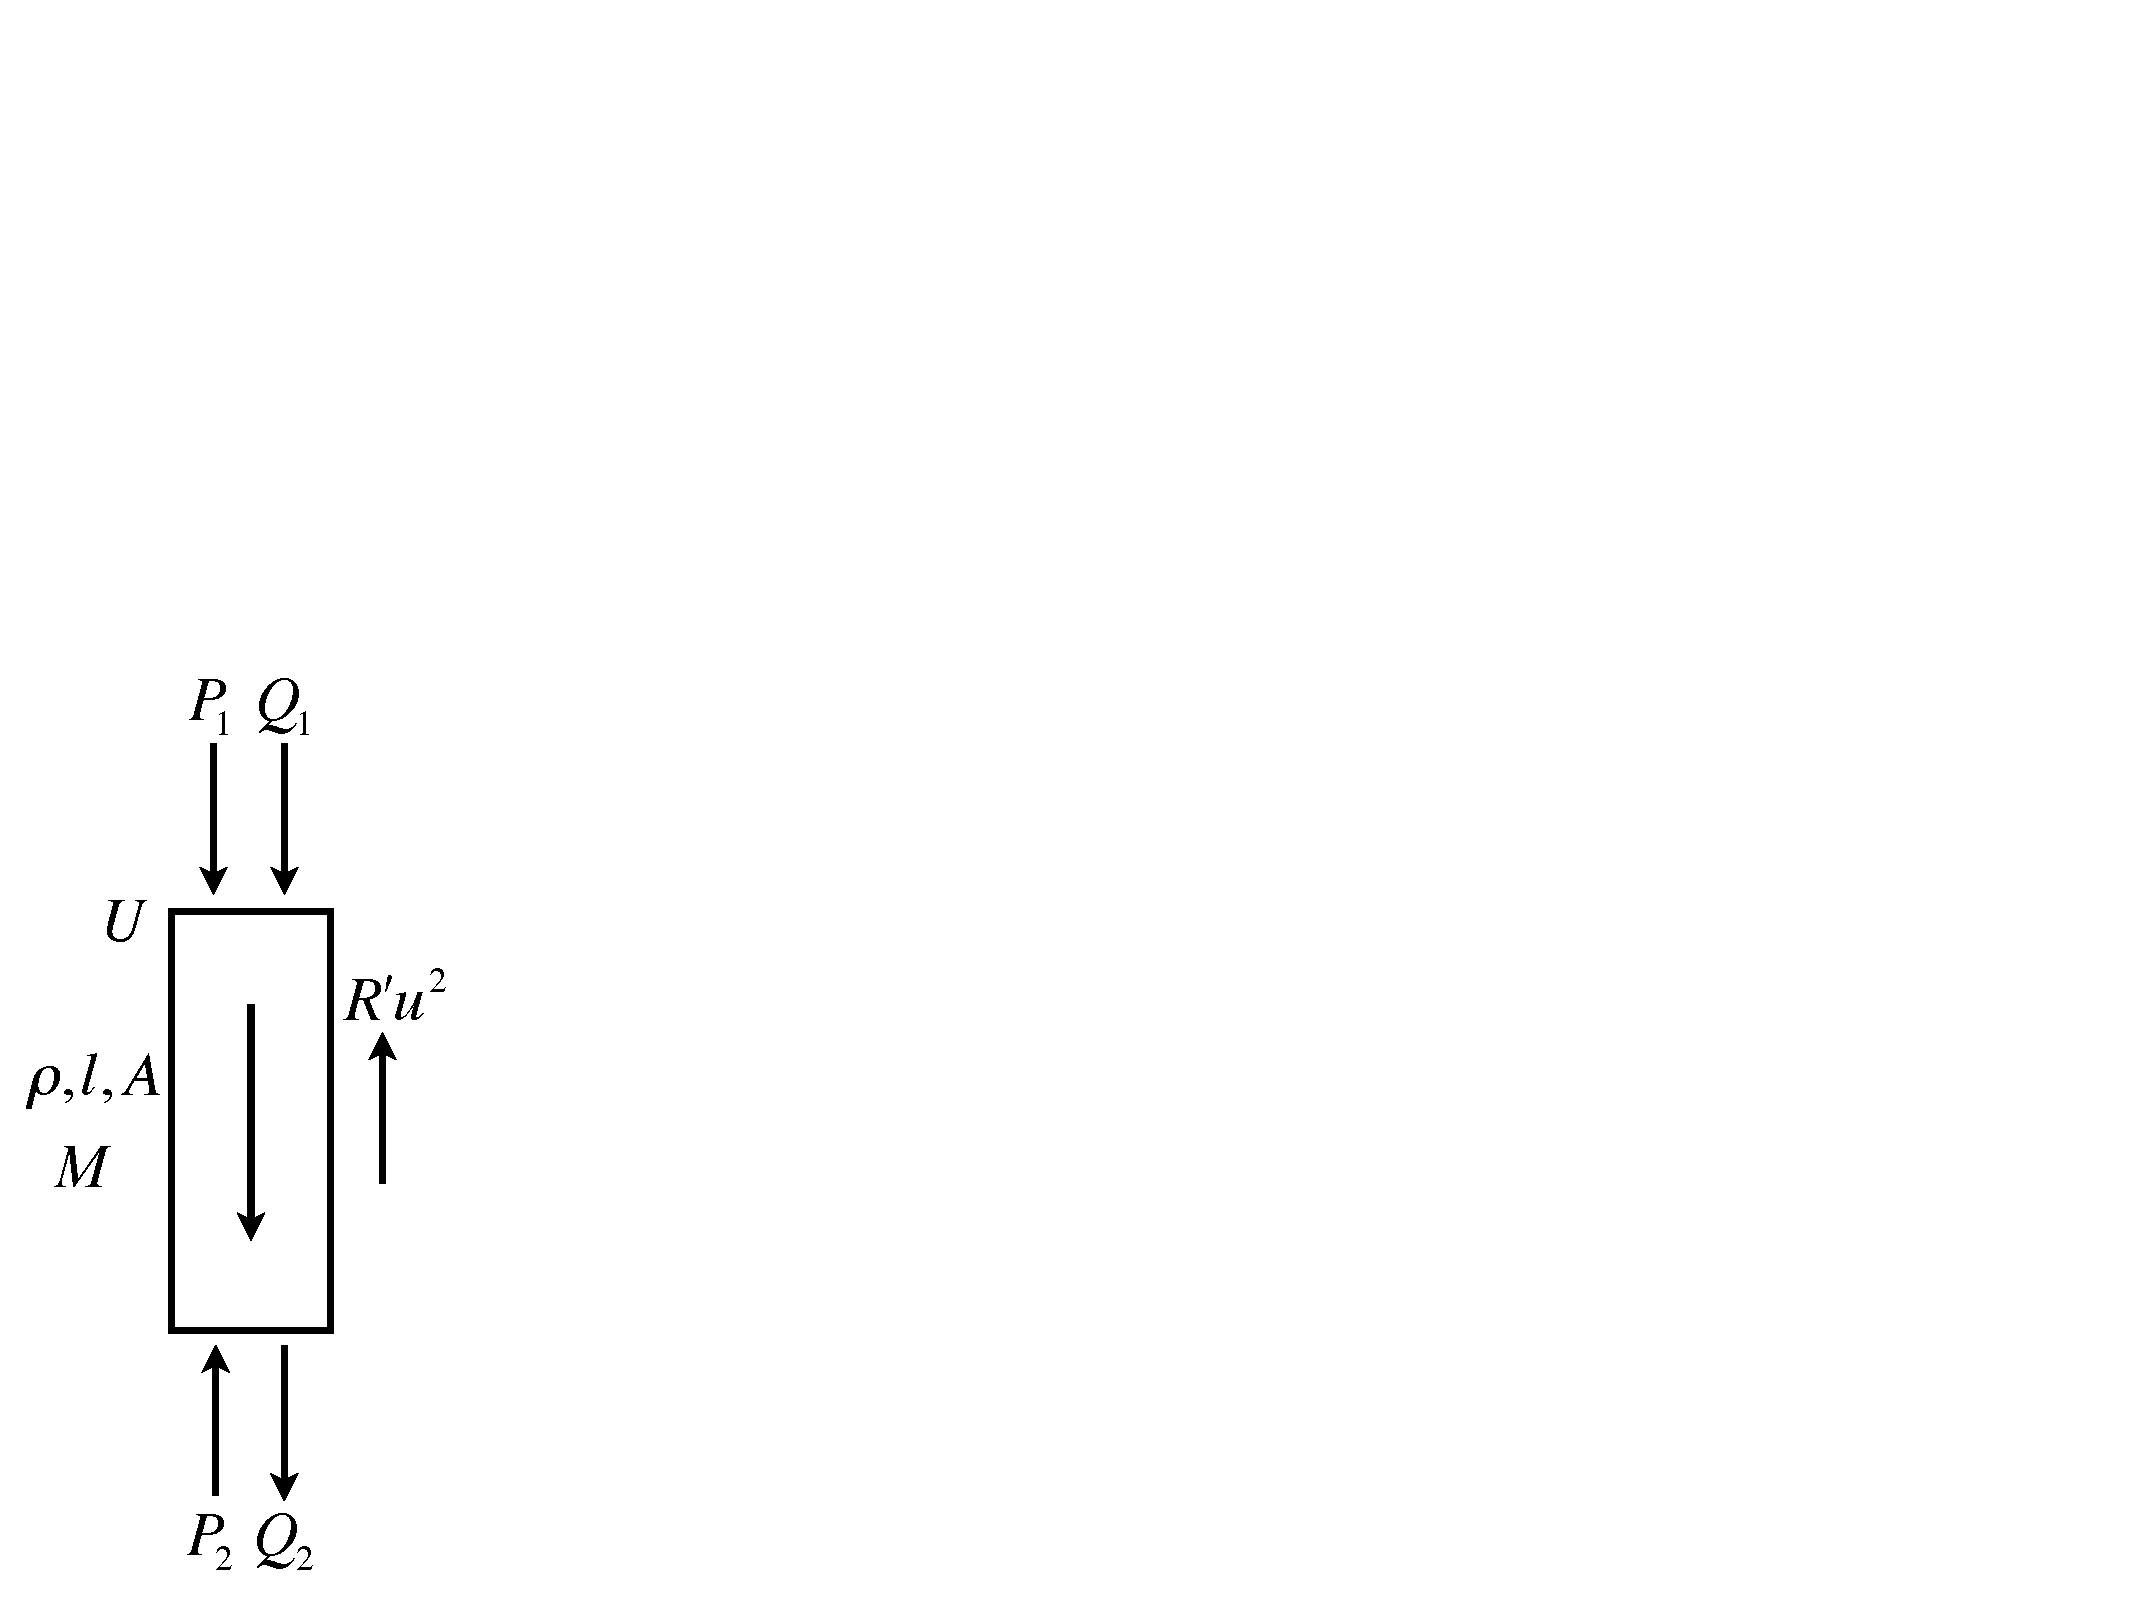
\includegraphics[width=1.2in]{Straight-Tube.pdf}
    \caption*{(a) 输液直管}
  \end{minipage}
  \centering
  \begin{minipage}[b]{0.3\textwidth}
    \centering
    %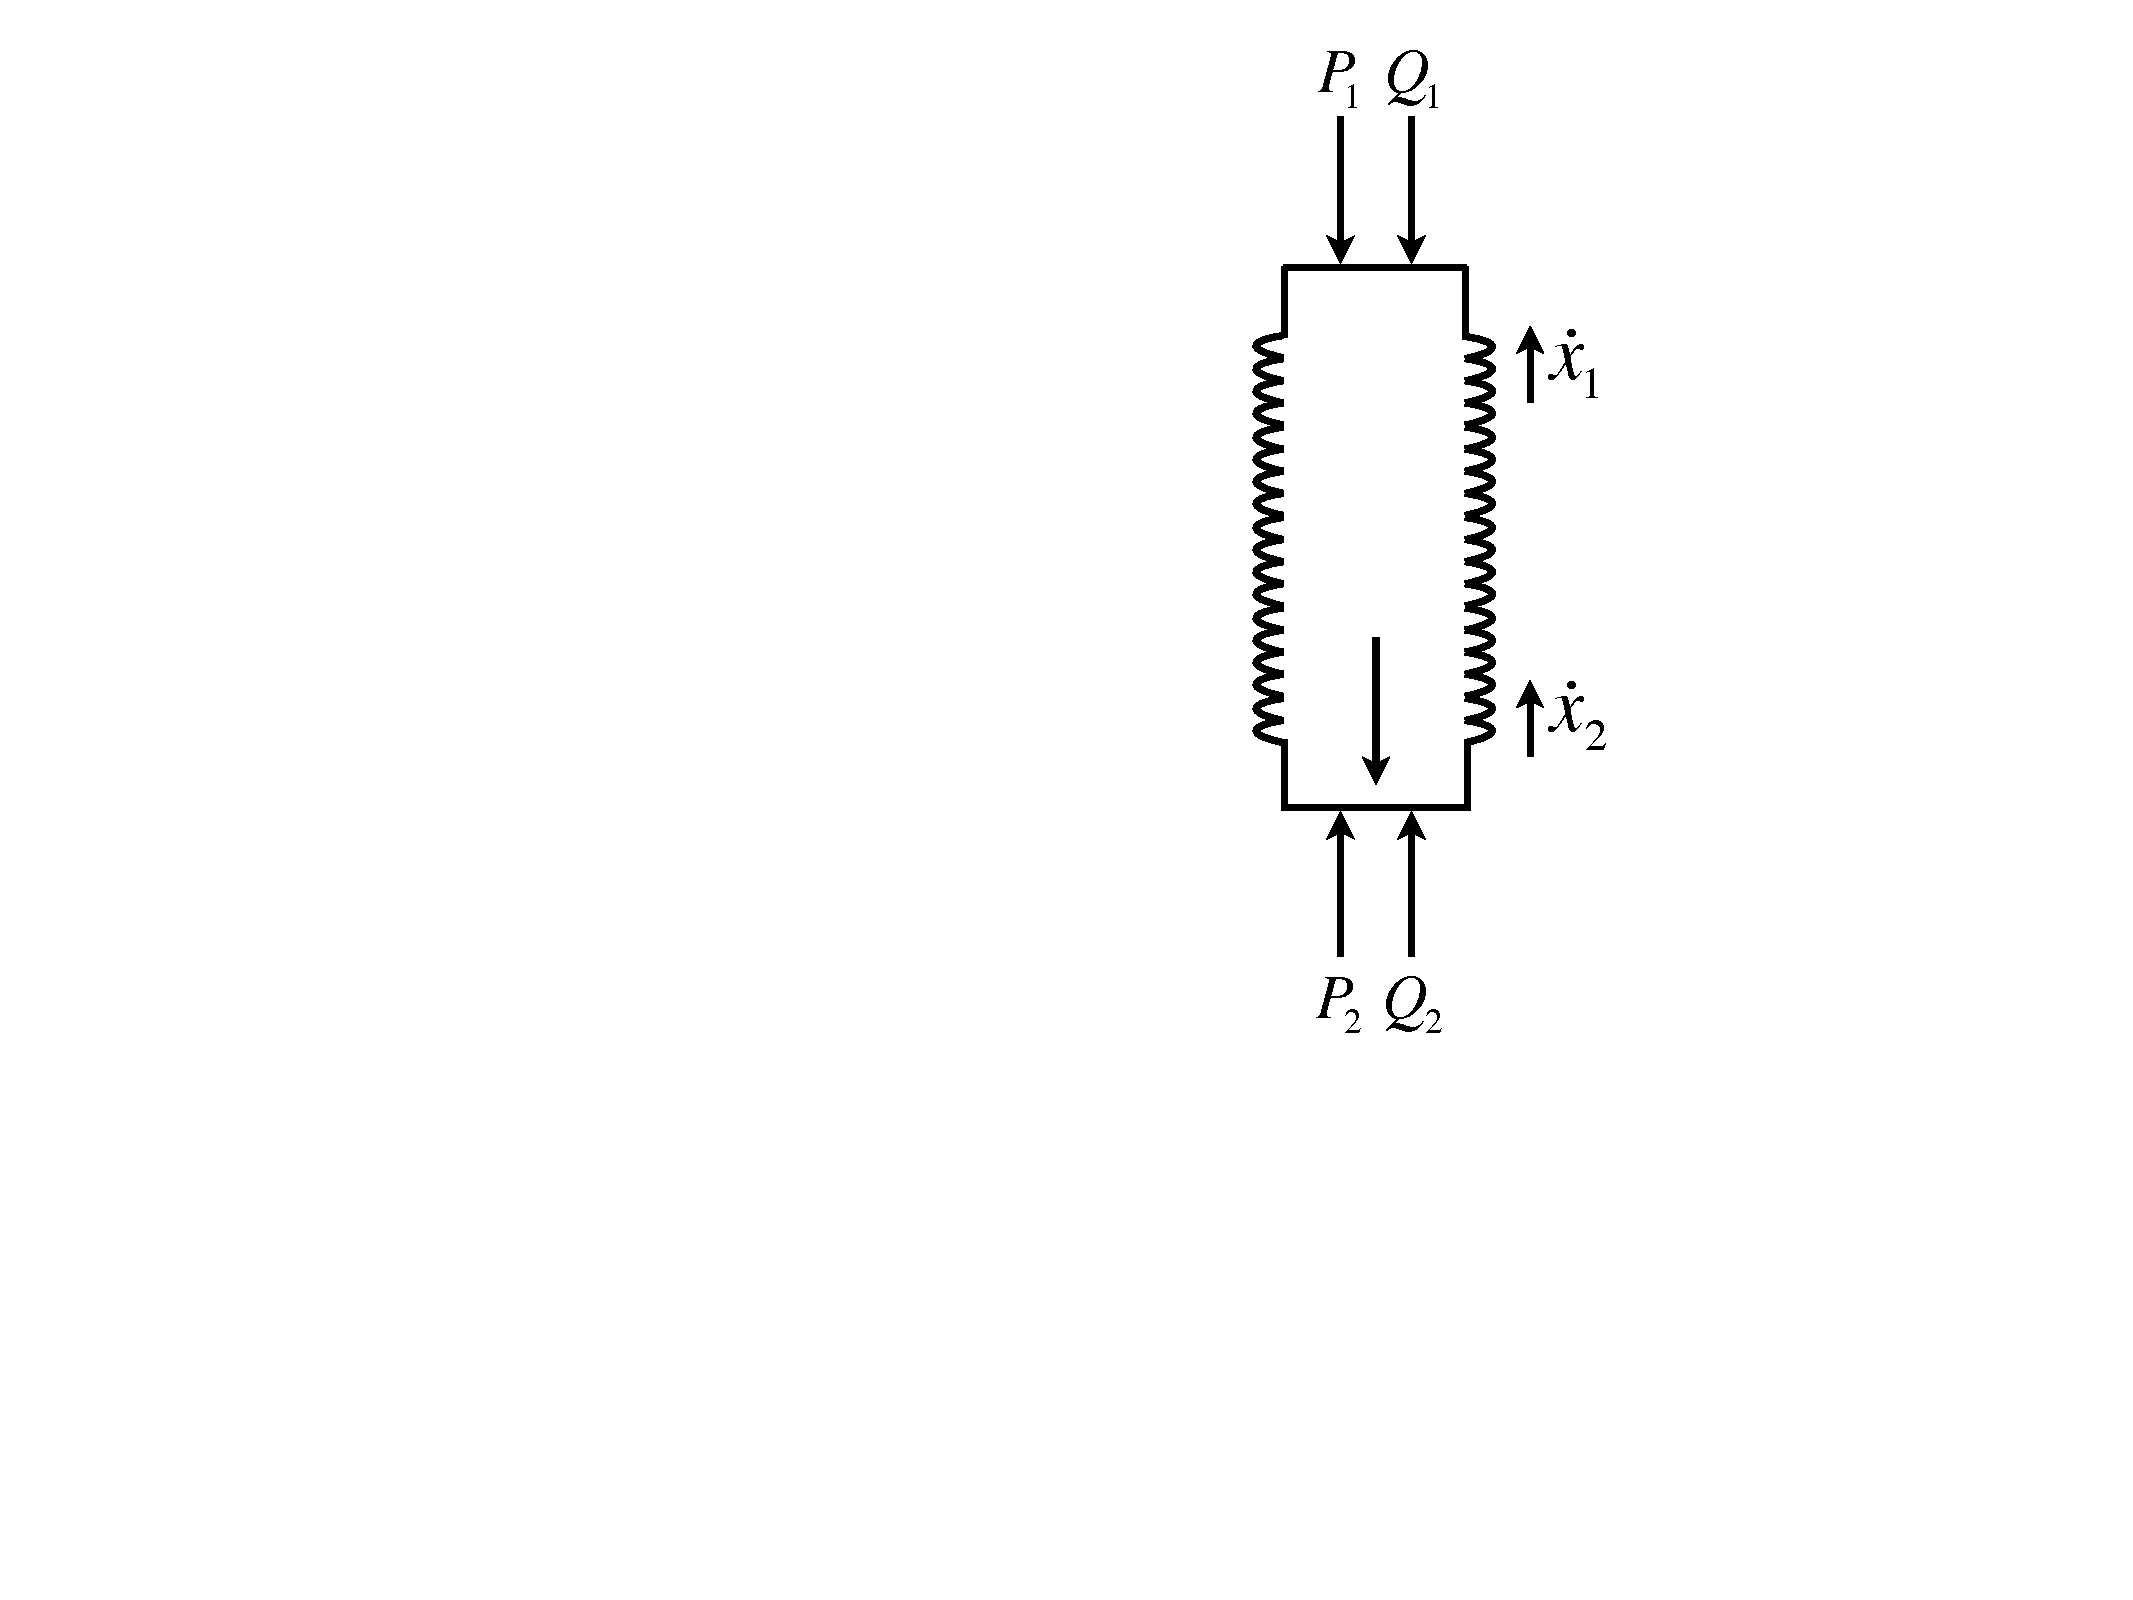
\includegraphics[width=1in]{Bellow.pdf}
    \caption*{(b) 波纹管}
  \end{minipage}
  \centering
  \begin{minipage}[b]{0.3\textwidth}
    \centering
    %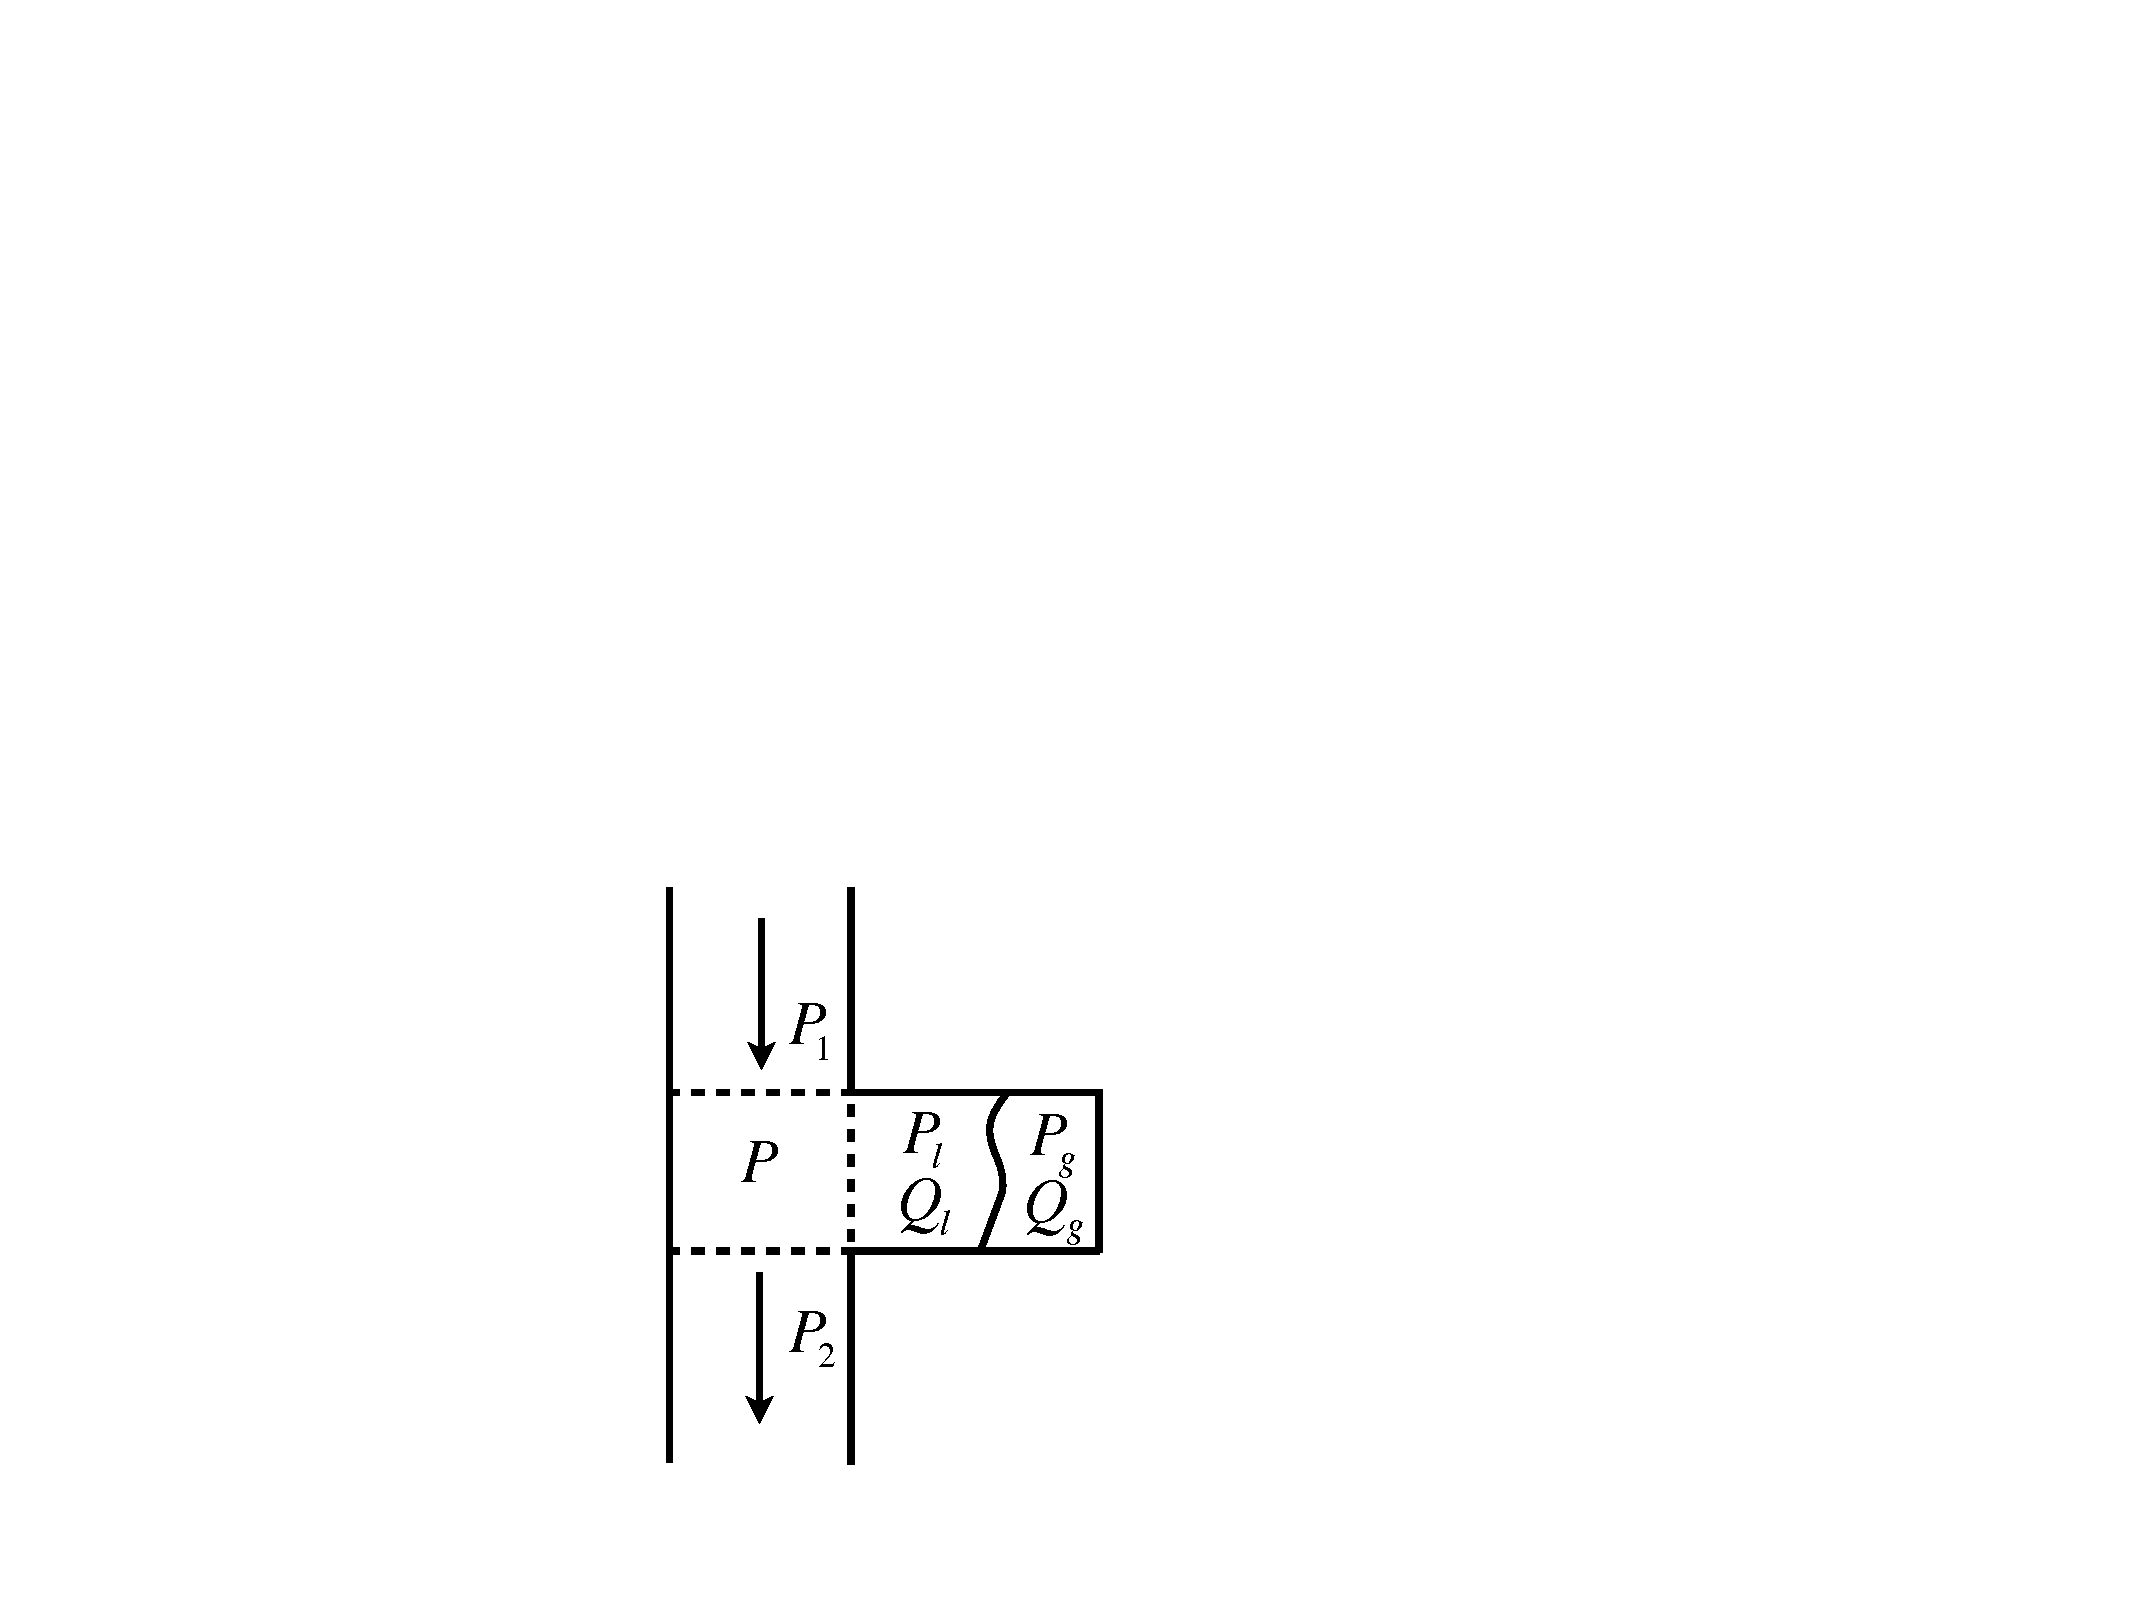
\includegraphics[width=1.5in]{Accumulator.pdf}
    \caption*{(c) 蓄压器}
  \end{minipage}
  \centering
  \begin{minipage}[b]{0.3\textwidth}
    \centering
    %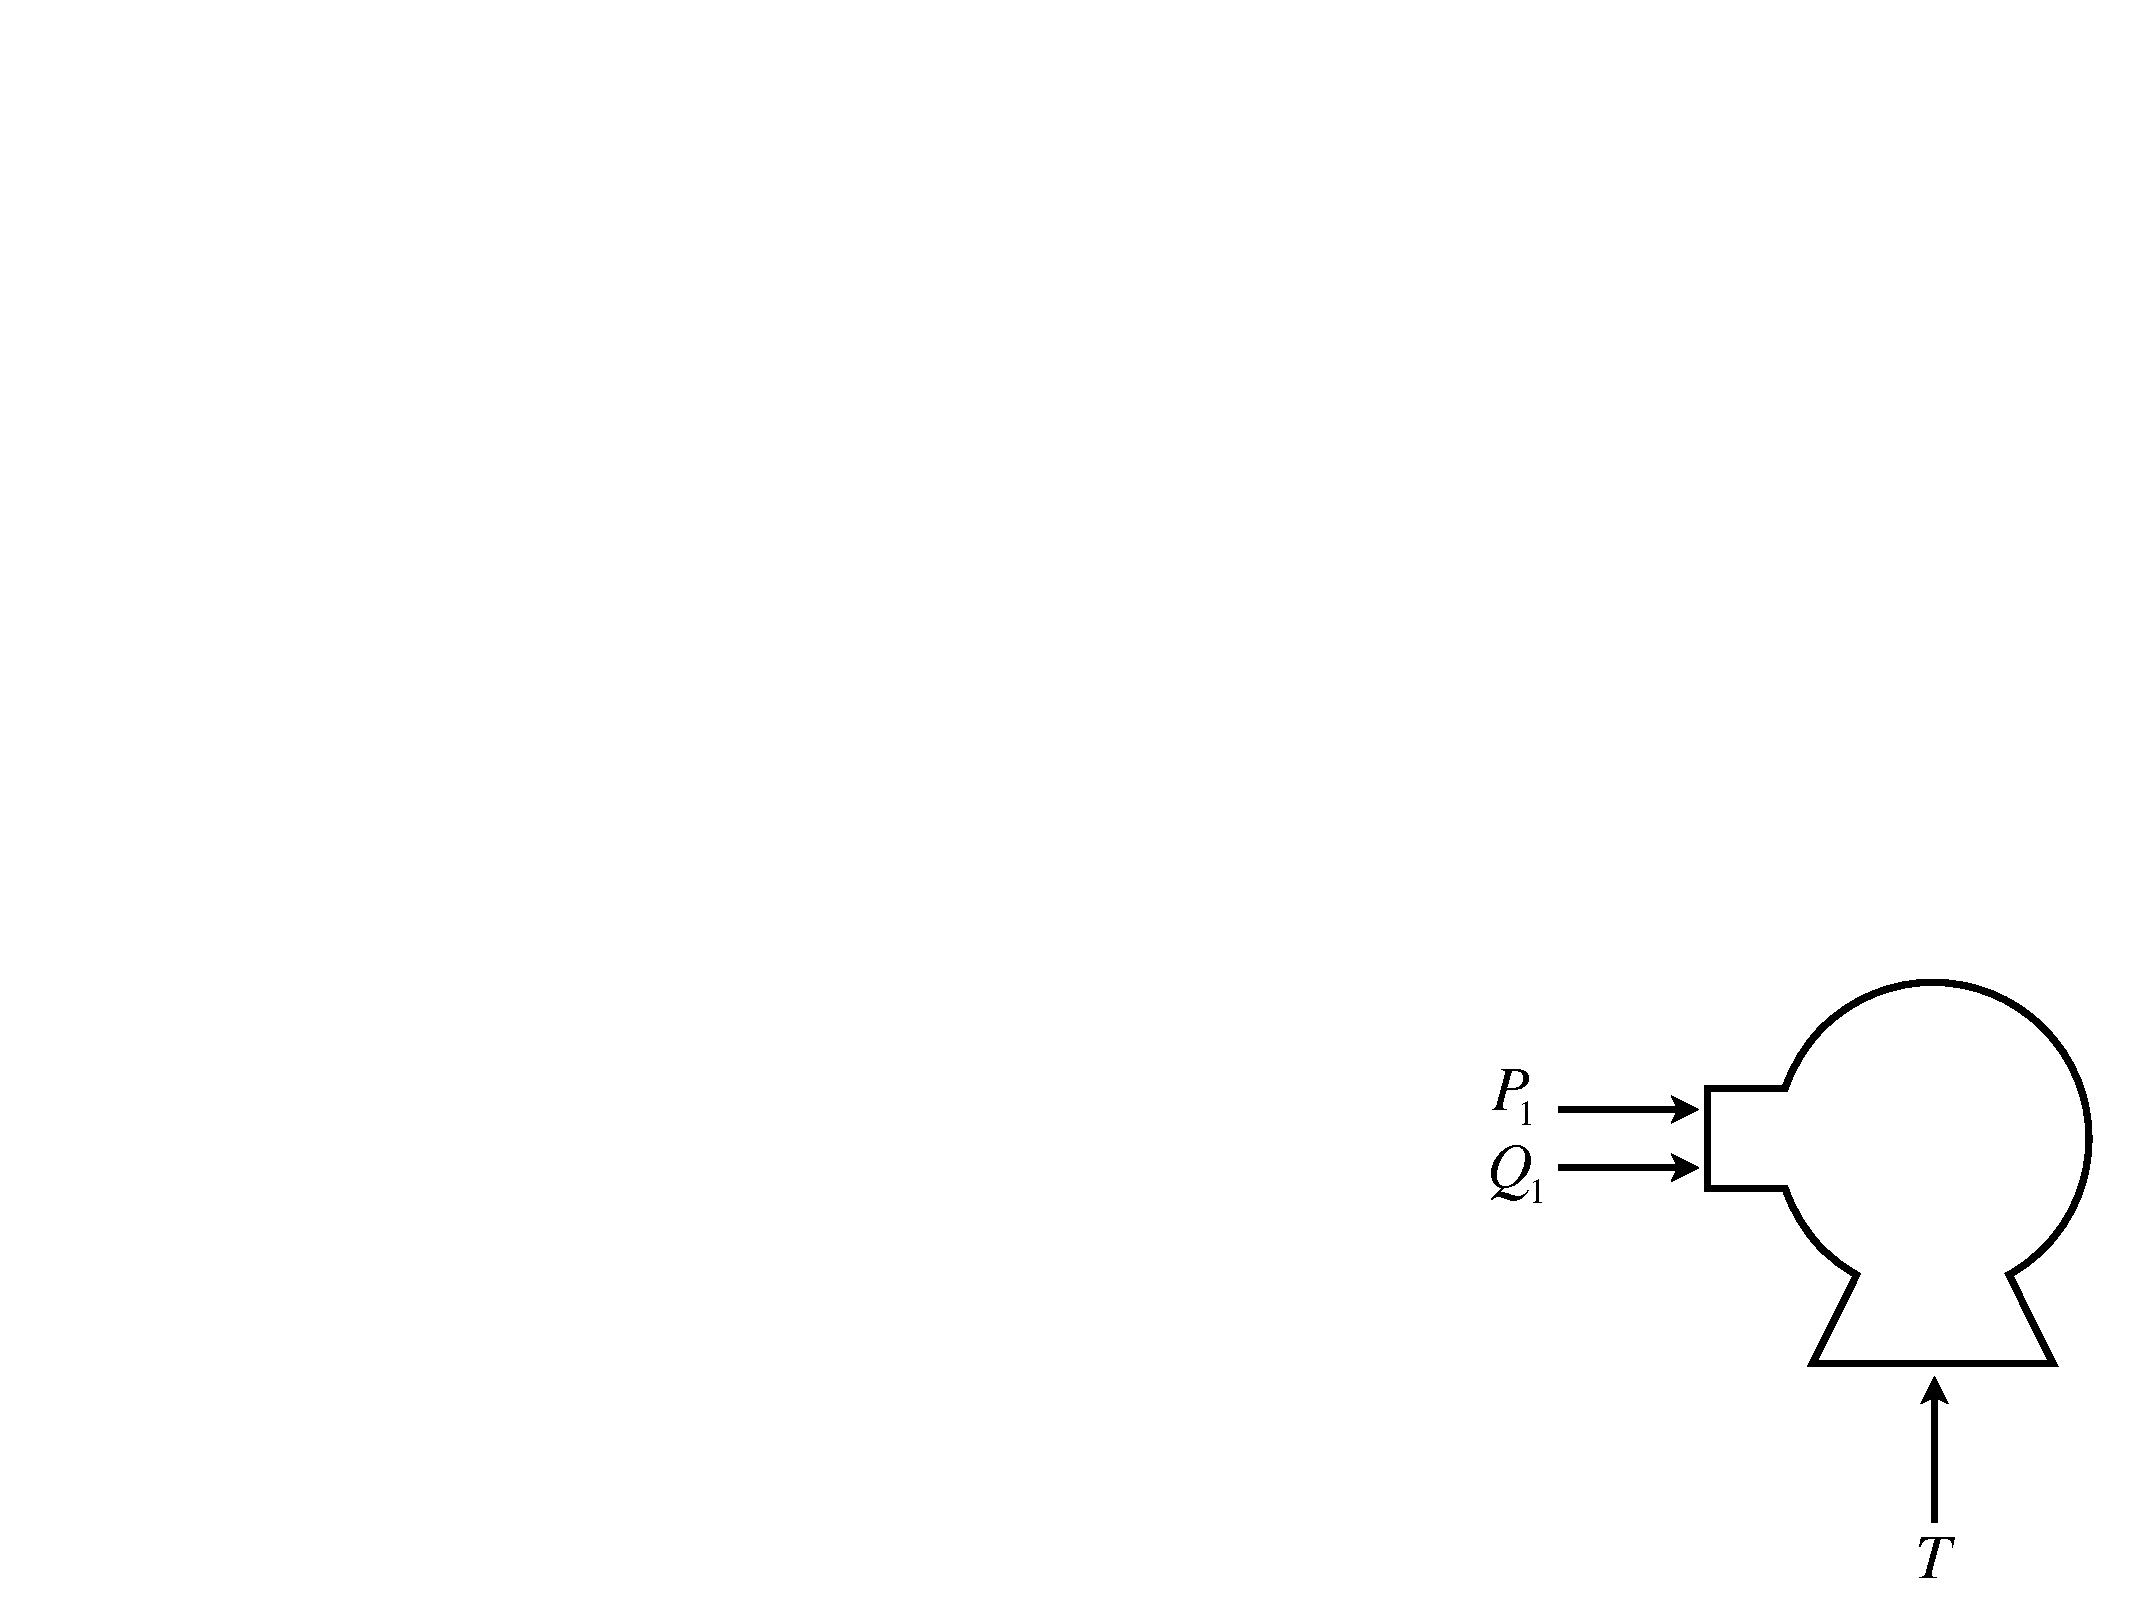
\includegraphics[width=1.6in]{Thrust.pdf}
    \caption*{(d) 推力室}
  \end{minipage}
  \centering
  \begin{minipage}[b]{0.3\textwidth}
    \centering
    % %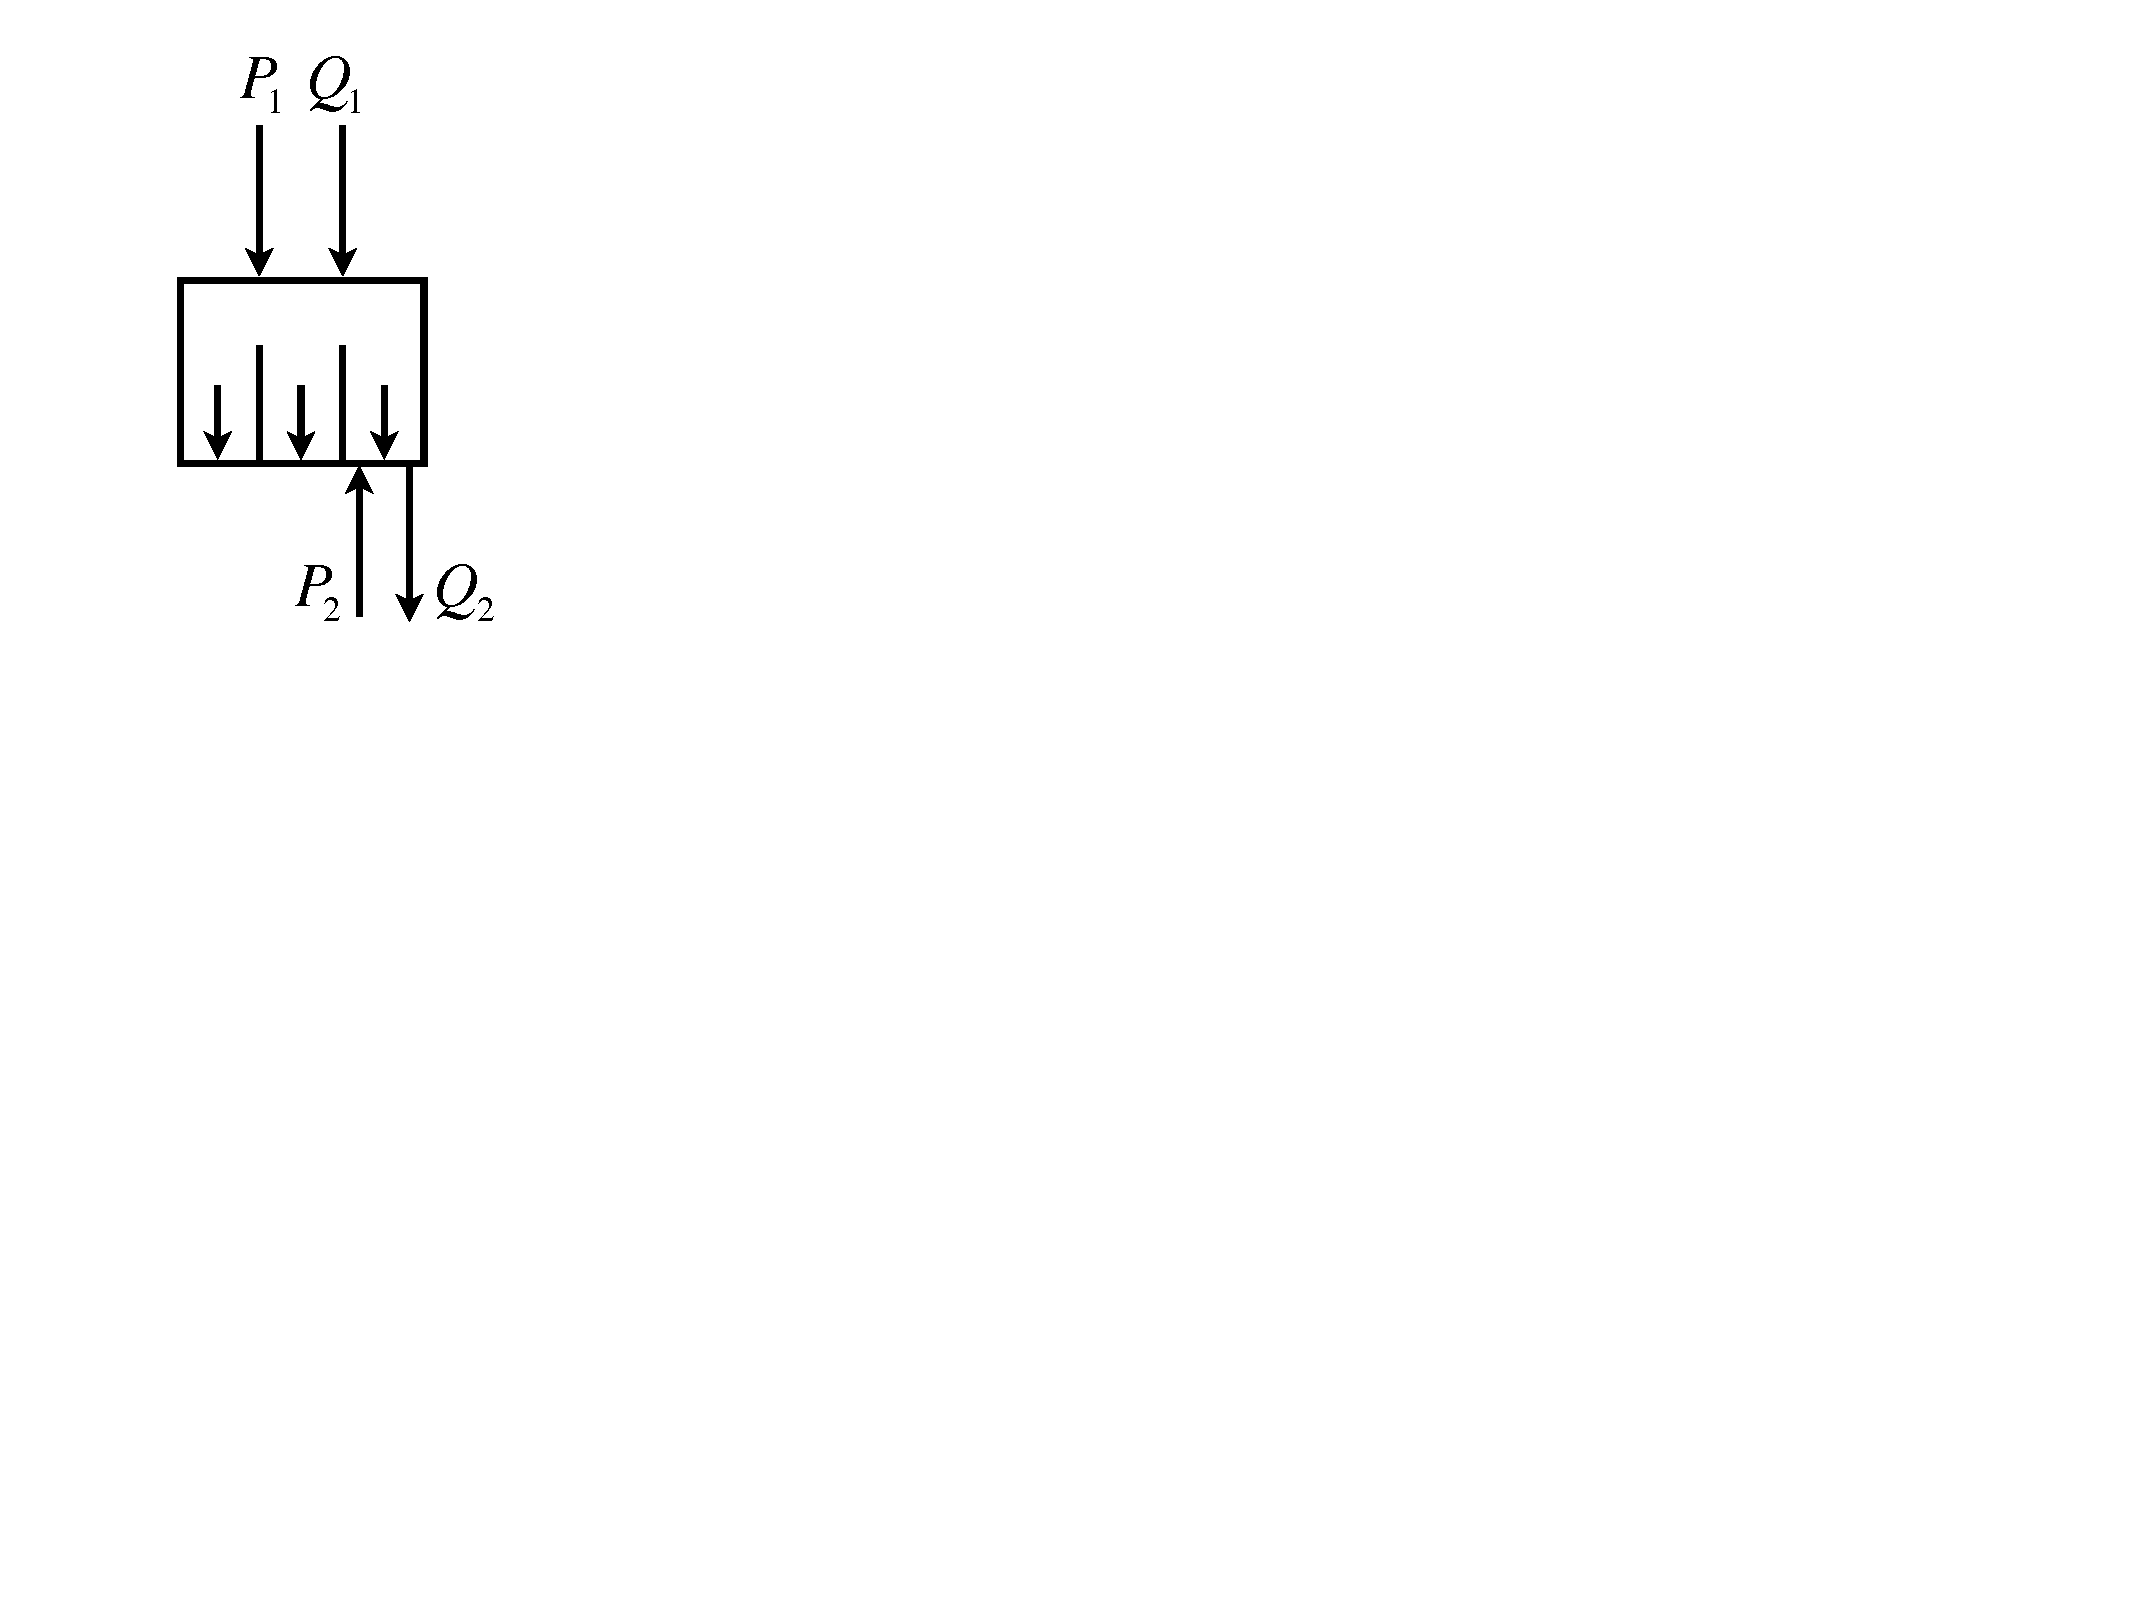
\includegraphics[width=1in]{Multiplex.pdf}
    \caption*{(e) 多通连接器}
  \end{minipage}
  \centering
  \begin{minipage}[b]{0.3\textwidth}
    \centering
    %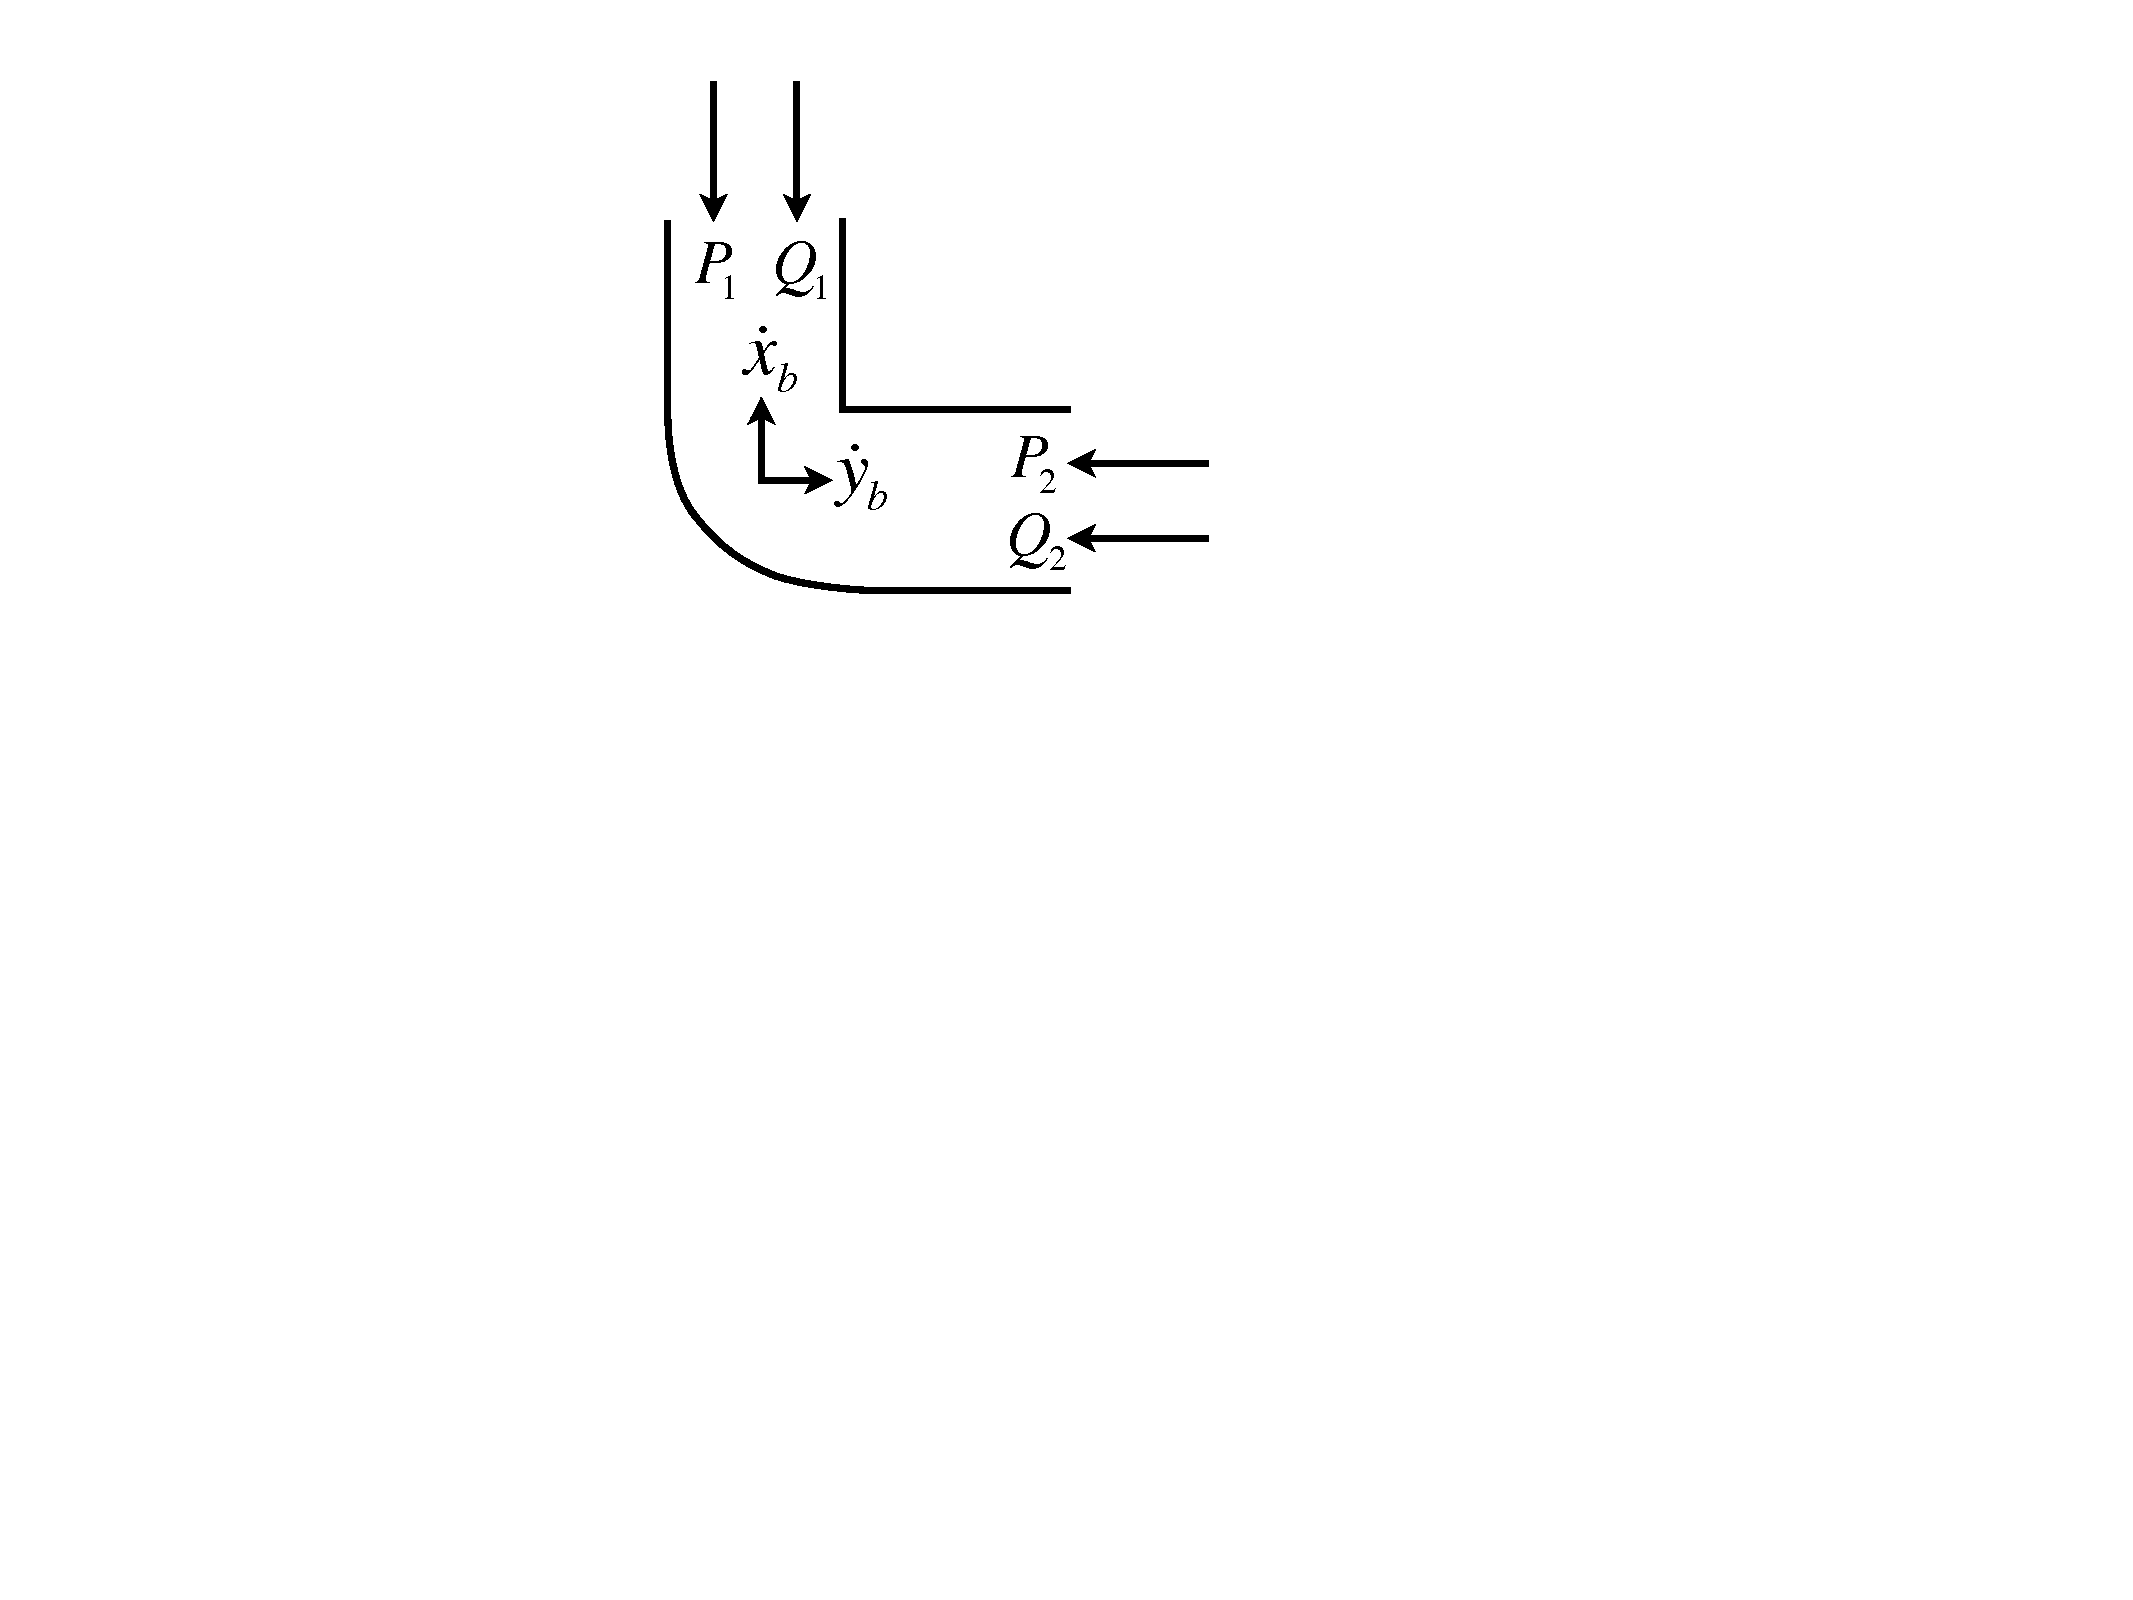
\includegraphics[width=1.7in]{Pump.pdf}
    \caption*{(f) 发动机泵}
  \end{minipage}
  \caption{液体火箭管路系统典型元件}
  \label{FeedLine-TypicalElement}
\end{figure}

液体推进火箭的管路系统主要由抽吸管路、多通接头、泵、泵后管路、燃烧室、推力室、蓄压器等几部分组成(如图\ref{FeedLine-TypicalElement})。分析液体火箭流体系统动特性的方法有很多,这里采用工程上常用的集中参数分析法,又称LRC等效电路分析法\cite{Dimaggio:1972, Vaage:1972, YangMing:2010}。本节主要针对包含四管发动机的推进系统展开分析。假设四管发动机系统的结构是对称的,并且流体的流动状态也是对称的,可以将四管发动机系统简化为单管发动机系统进行处理。单管发动机管路系统各元件之间脉动压力和脉动流量的传递关系如图\ref{POGO-PipeLine}所示。

\begin{figure}[!htb]
  \centering
  %%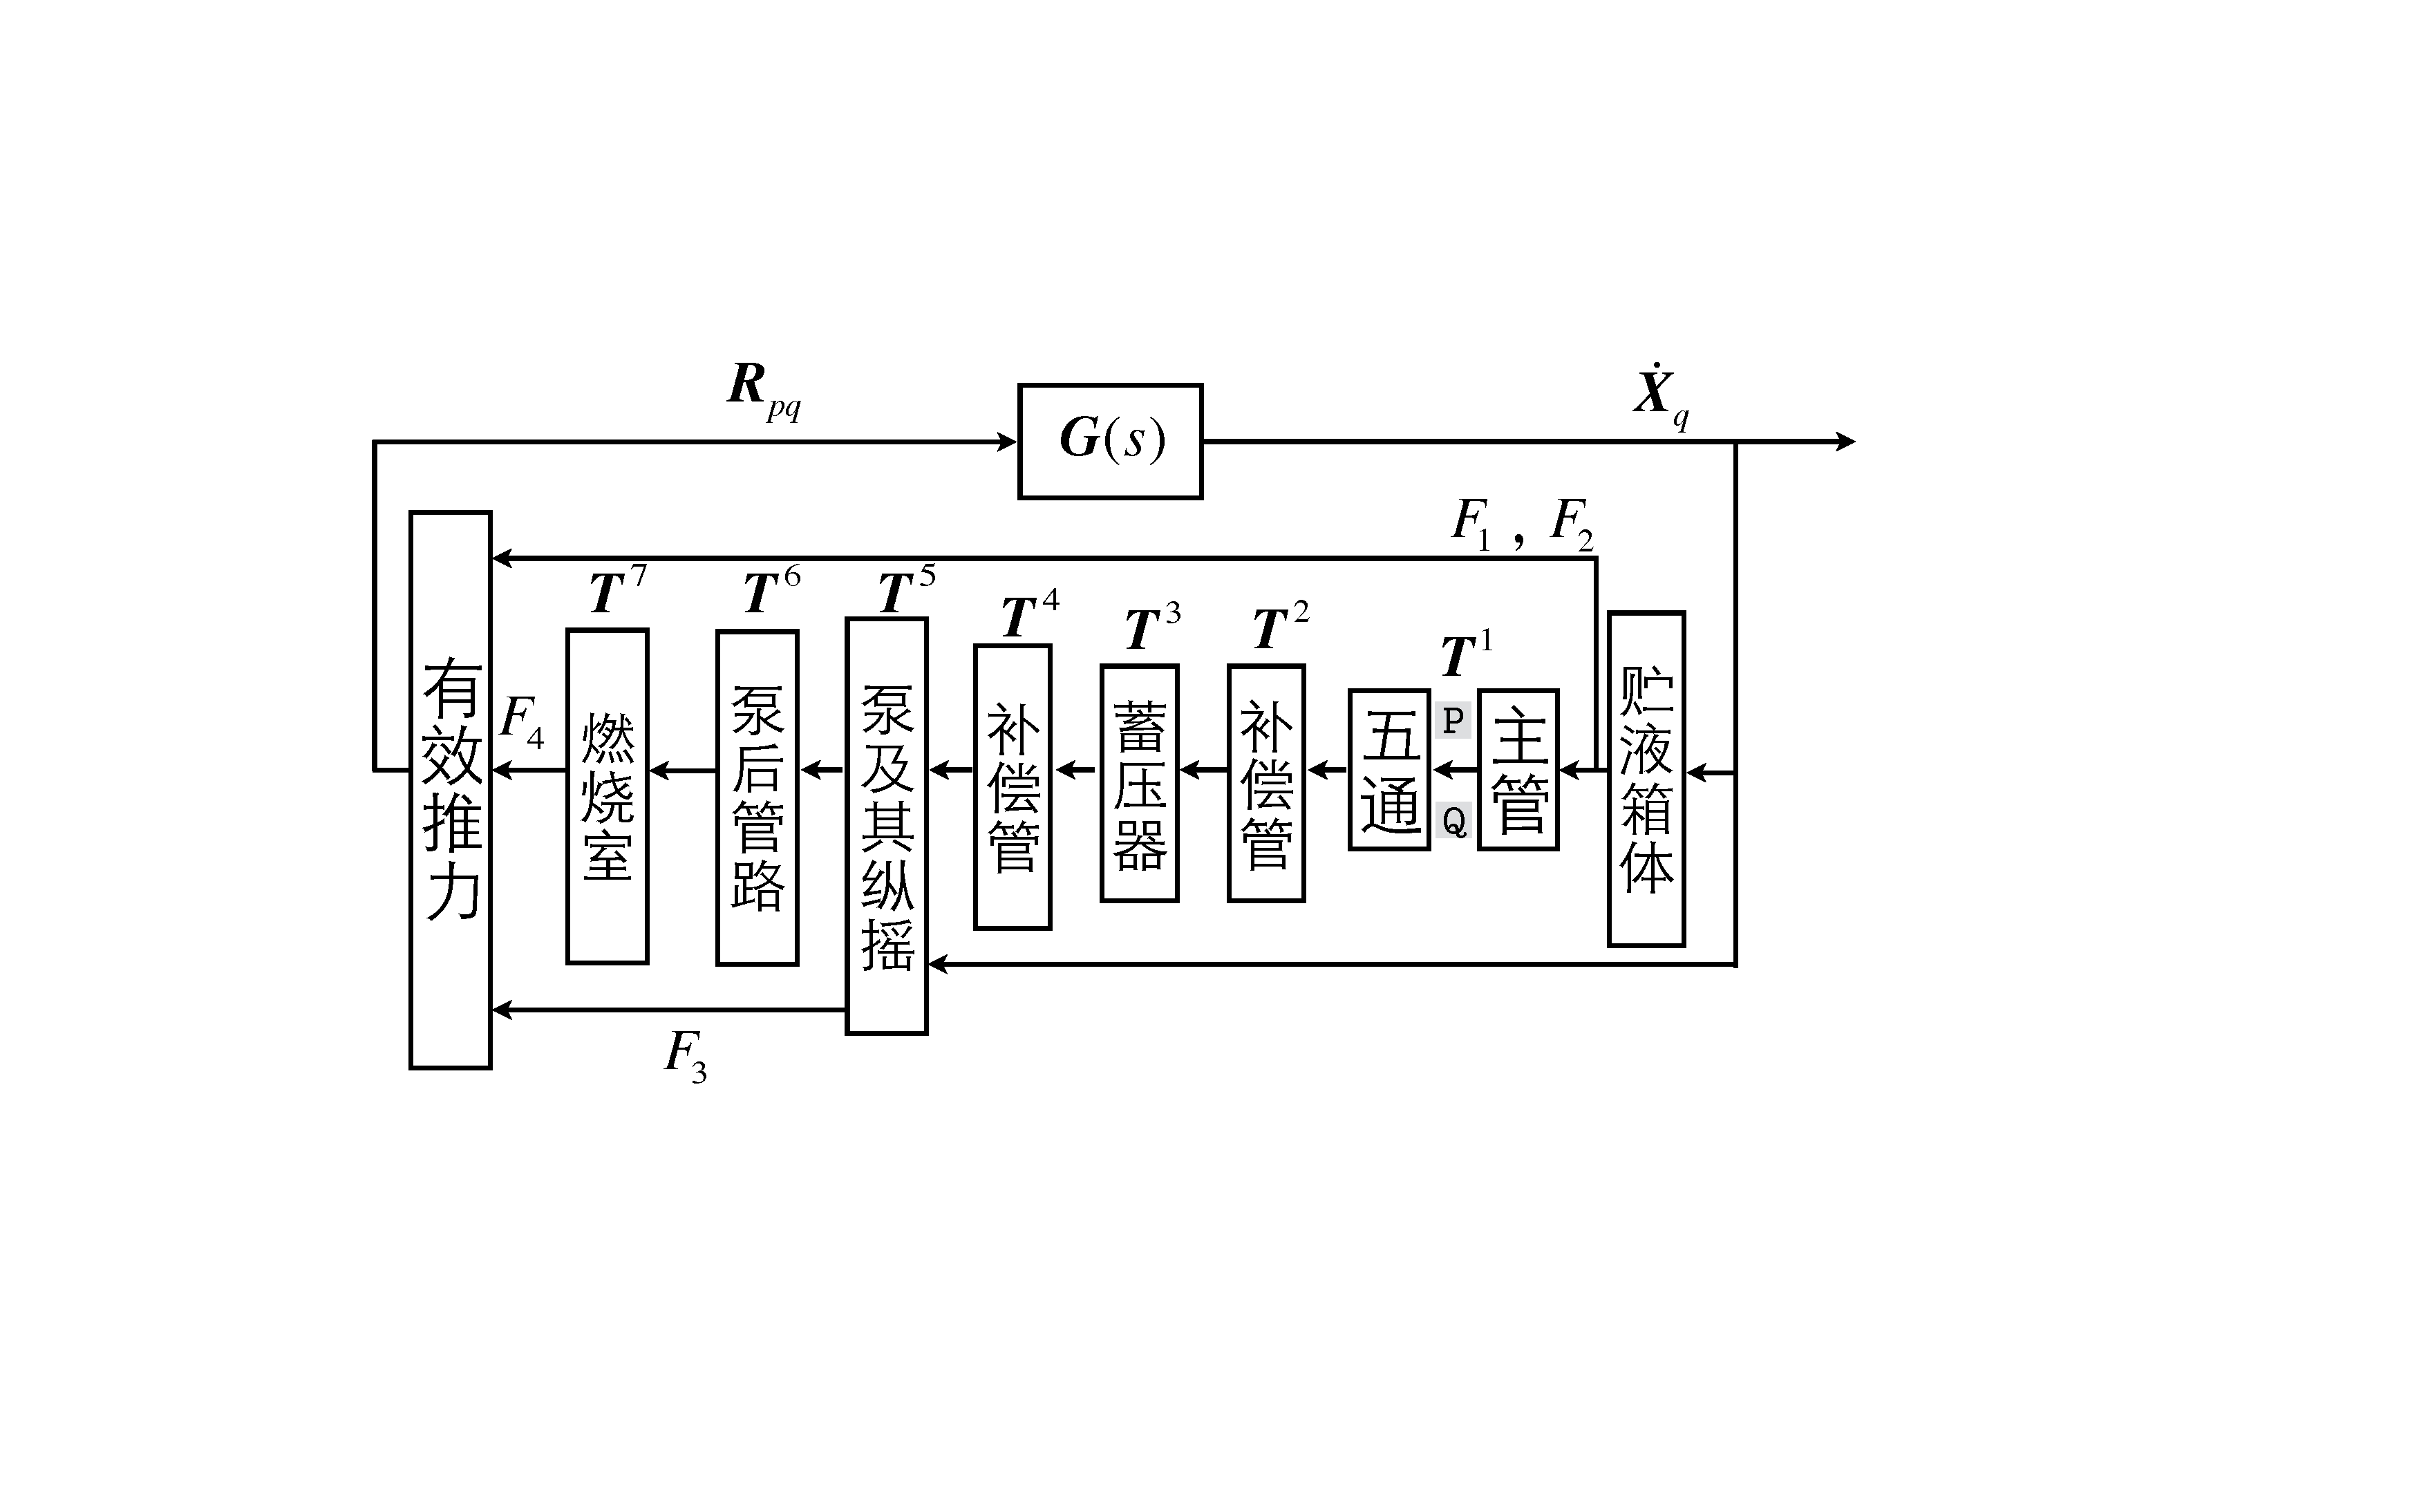
\includegraphics[width=.9\linewidth]{PipeLines.pdf}
  \caption{液体火箭管路-结构耦合系统传递关系示意图}\label{POGO-PipeLine}
\end{figure}

\begin{enumerate}[label=\textbf{\Roman*.}, align=left, leftmargin=0pt, listparindent=\parindent, itemindent=!, labelwidth=\parindent, labelsep=0pt, itemsep=1em]
  \litem{输液直管}
  由于通常情况下输液直管的直径与长度之比很小,所以在研究其低频振动时,可以不考虑管两端的复杂现象,仅考虑液体的一维流动。管中液体的扰动可以用欧拉方程和连续性方程来描述:
  \begin{align}
    \frac{\partial v}{\partial t}+{{v}_{0}}\frac{\partial v}{\partial x}+\frac{1}{\rho }\frac{\partial p}{\partial x} & =0 \nonumber \\
    \frac{\partial p}{\partial t}+{{v}_{0}}\frac{\partial p}{\partial x}+c_{0}^{2}\rho \frac{\partial v}{\partial x}  & =0
  \end{align}
  其中$v_0,c_0$为未扰动流的速度和当地声速,$p(x,t),v(x,t)$为流体的脉动压力和脉动速度。对上式进行求解,经过推导可以得到如下的输液直管上、下游脉动压力和流量之间的传递关系式:
  \begin{equation}
    \label{eq:Straight-Tube}
    \left[ \begin{matrix}
        {{P}_{2}} \\
        {{Q}_{2}} \\
      \end{matrix} \right]=\left[ \begin{matrix}
        \cosh \left( \theta  \right)                                   & {\displaystyle -\frac{Z\sinh \left( \theta  \right)}{\theta }} \\
        {\displaystyle -\frac{\theta \sinh \left( \theta  \right)}{Z}} & \cosh \left( \theta  \right)                                   \\
      \end{matrix} \right]\left[ \begin{matrix}
        {{P}_{1}} \\
        {{Q}_{1}} \\
      \end{matrix} \right]
  \end{equation}
  式中$Z=sL+R,L=\rho l/A,\tau =lc,\theta^2=s^2\tau^2Z/(sL)$,其中$l$为管路长度,$Z$为液路阻抗,$L$为液路惯性,$R$为液路阻力,$c$为当地声速,$\rho$为液体密度,$s$为拉普拉斯变量,$A$为管路截面积。

  \litem{蓄压器动力学模型}蓄压器是典型的POGO振动抑制器件,这里主要介绍目前国内外广泛应用的被动封闭式蓄压器,其简化物理模型如图\ref{FeedLine-TypicalElement}(c)所示。这种蓄压器包括了气腔和液腔,假设内部气体满足多方气体定律$P_gV_g^{\gamma}=C_g$,模拟输液直管传递关系的推导方法,可以得出其如下的传递关系:
  \begin{equation}
    \left[ \begin{matrix}
        {P_2} \\
        {Q_2} \\
      \end{matrix} \right]=\left[ \begin{matrix}
        1  & 0 \\
        -Y & 1 \\
      \end{matrix} \right]\left[ \begin{matrix}
        {P_1} \\
        {Q_1} \\
      \end{matrix} \right]
  \end{equation}
  记蓄压器阻抗为$Z$、导纳为$Y$
  \begin{align}
    Z & =\frac{s^2CL+sCR+1}{sC} \nonumber                                                         \\
    Y & =\frac{1}{Z}=\frac{s}{\displaystyle L\left(s^2+2\zeta\omega s+\omega^2 \right)} \nonumber
  \end{align}
  其中$\omega=\sqrt{1/CL},\zeta=CR\omega/2$,$C$为蓄压器柔度,$R$和$L$意义同上。
\end{enumerate}

至此,可以利用上述管段元件的传递关系进行液体火箭管路系统的总体传递矩阵组装(矩阵记号参考图\ref{POGO-PipeLine})
\begin{equation}
  \boldsymbol{\mathbb{T}}=\boldsymbol{T}^6\boldsymbol{T}^5\boldsymbol{T}^4\boldsymbol{T}^3\boldsymbol{T}^2\boldsymbol{T}^1=\left[ \begin{matrix}
      {T}_{11} & {T}_{12} \\
      {T}_{21} & {T}_{22} \\
    \end{matrix} \right],\;
  \boldsymbol{T}^s=\boldsymbol{T}^6 \left[
    \begin{matrix}
      -A_{L1}^{(5)}Z_{L1}^{(5)} \\
      A_{L1}^{(5)}              \\
    \end{matrix} \right] = \left[ \begin{matrix}
      {T}_{1}^s \\
      {T}_{2}^s \\
    \end{matrix} \right]
\end{equation}
考虑管路系统入口处脉动压力和脉动流量与箱底振动速度之间的关系:
\begin{equation}
  \label{eq:Inlet-Boundary-Condition}
  P_{L1}^{(1)}=s\rho{h}_T\left(1-\frac{A_{L1}^{(1)}}{A_T}\right){\dot{x}_T}(s)- \frac{s\rho{h_T}Q_{L1}^{(1)}}{A_T}
\end{equation}
其中,符号下标${}_{L1},{}_{L2}$用于区分管路参数描述位置(入口或出口),数字上标${}^{(n)}$表示该参数描述第$n$段管路元件, $h_T$为贮箱液面高度,$A_{L1}^{(1)}, A_T$分别表示与贮箱底部相连管路的截面积和贮箱截面积,$\dot{x}_T$表示箱底扰动速度。

结合发动机燃烧室内的压力上下游平衡关系$P_{L1}^{(7)}=P_{L2}^{(6)}$,经过一系列换算,最终可以得到管路系统初始脉动压力$P_{L1}^{(1)}$和脉动流量$Q_{L1}^{(1)}$与箱底扰动速度$\dot{x}_T$和泵位置扰动速度$\dot{x}_{L1}^{(5)}$之间的传递关系:
\begin{align}
  \label{eq:Total-Transfer}
  Q_{L1}^{(1)}= & \frac{\left( {T}_{1}^{s}-Z_{L1}^{(7)} {T}_{2}^{s} \right)\dot{x}_{L1}^{(5)}(s)- s{\rho}{h_T}\left( 1- {\displaystyle \frac{A_{L1}^{(1)}}{A_T}} \right) \left( Z_{L1}^{(7)} {T}_{21}- {T}_{11} \right) {\dot{x}_T(s)} } {Z_{L1}^{(7)} {T}_{22}- {T}_{12}- {\displaystyle \frac{s\rho h_T}{A_T}} \left( Z_{L1}^{(7)} {T}_{21}- {T}_{11} \right)} \nonumber \\
  %%%
  P_{L1}^{(1)}=% 
                & -\frac{s\rho{h_T}}{A_T} \left[
  \frac{\left( {T}_{1}^{s}-Z_{L1}^{(7)} {T}_{2}^{s} \right)\dot{x}_{L1}^{(5)}(s)- s{\rho}{h_T}\left( 1- { \frac{A_{L1}^{(1)}}{A_T}} \right) \left( Z_{L1}^{(7)} {T}_{21}- {T}_{11} \right) {\dot{x}_T(s)} } {Z_{L1}^{(7)} {T}_{22}- {T}_{12}- { \frac{s\rho h_T}{A_T}} \left( Z_{L1}^{(7)} {T}_{21}- {T}_{11} \right)}
  \right] \nonumber                                                                                                                                                                                                                                                                                                                                                        \\
                & + s\rho{h}_T \left(1- \frac{A_{L1}^{(1)}}{A_T}\right){\dot{x}_T}(s)
\end{align}

通常,作用在液体火箭上的典型外力主要包括了以下几类:\label{Page:Typical-Feedback-Force}
\begin{enumerate}[leftmargin=\parindent, align=parleft, labelindent=0pt, labelwidth=*]
  \item 贮箱底开口处相对脉动流出量引起贮箱液体质心脉动对结构作用力。
        \begin{equation}
          F_1=\rho h_Ts \left[ Q_{L1}^{(1)}+ A_{L1}^{(1)}\dot{x}_T(s) \right]
        \end{equation}
  \item 贮箱底开口处的脉动压力对结构作用力。
        \begin{equation}
          F_2=A_{L1}^{(1)}P_{L1}^{(1)}
        \end{equation}
  \item 泵前后压力动量变化对结构作用力。
        \begin{equation}
          F_3=N\left[ -A_{L1}^{(4)}P_{L1}^{(5)}- \rho Q_s \left( \frac{2Q_{L1}^{(5)}}{A_{L1}^{(4)}}+ \dot{x}_{L1}^{(5)}(s) \right)\right]
        \end{equation}
  \item 发动机燃烧室脉动压力引起脉动推力。
        \begin{equation}
          F_4=NA_{th}C_f P_{L2}^{(7)}
        \end{equation}
\end{enumerate}
其中,$A_{L1}^{(4)}$表示泵上游入口处截面积,$Q_s$表示泵的稳态体积流,$N$表示发动机台数,$A_{th}$为发动机喉部截面积,$C_f$为有效推力系数。

利用公式\eqref{eq:Total-Transfer},可以把管路推进系统作用到结构上的反馈力表示为:
\begin{equation}
  \label{eq:Feedback-Force-Transfer}
  \boldsymbol{F}_p(s)=\left[ \begin{matrix}
      F_1(s) \\
      F_2(s) \\
      F_3(s) \\
      F_4(s) \\
    \end{matrix} \right]  \triangleq \boldsymbol{R}_{pq}(s)\left[ \begin{matrix}
      \dot{x}_T(s)          \\
      \dot{x}_{L1}^{(5)}(s) \\
    \end{matrix} \right] \triangleq \boldsymbol{R}_{pq}(s)\boldsymbol{\dot{X}}_q(s)
\end{equation}
矩阵$\boldsymbol{R}_{pq}(s)$代表了箭体振动速度$\boldsymbol{\dot{X}}_q(s)$与推进系统反馈力$\boldsymbol{F}_p(s)$之间的传递关系。可以看出,该速度阻抗矩阵形式复杂,且包含了难以处理的超越函数。

\section{液体火箭结构系统集中参数模型}
\label{sec:Lumped-Rocket-Structural-System}
\begin{figure}[!htb]
  \centering
  %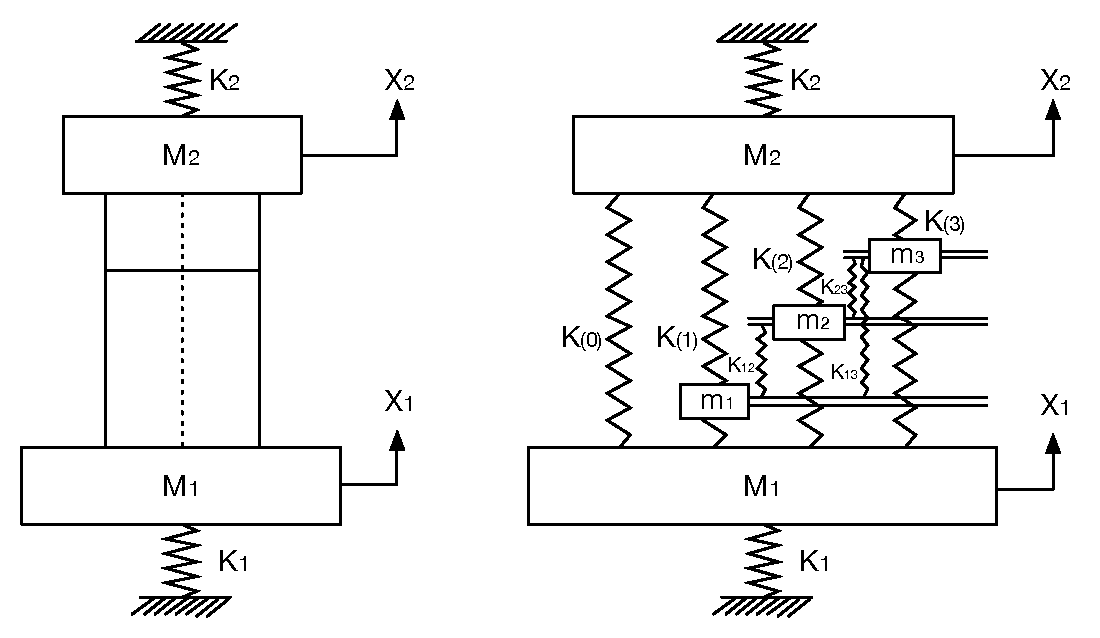
\includegraphics[width=.8\linewidth]{Lumped-Mass-Spring-Glaser}
  \caption{液体贮箱集中参数Glaser弹簧-质量模型}\label{Lumped-Mass-Spring-Glaser}
\end{figure}

\begin{figure}[p]
  \centering
  \centerline{%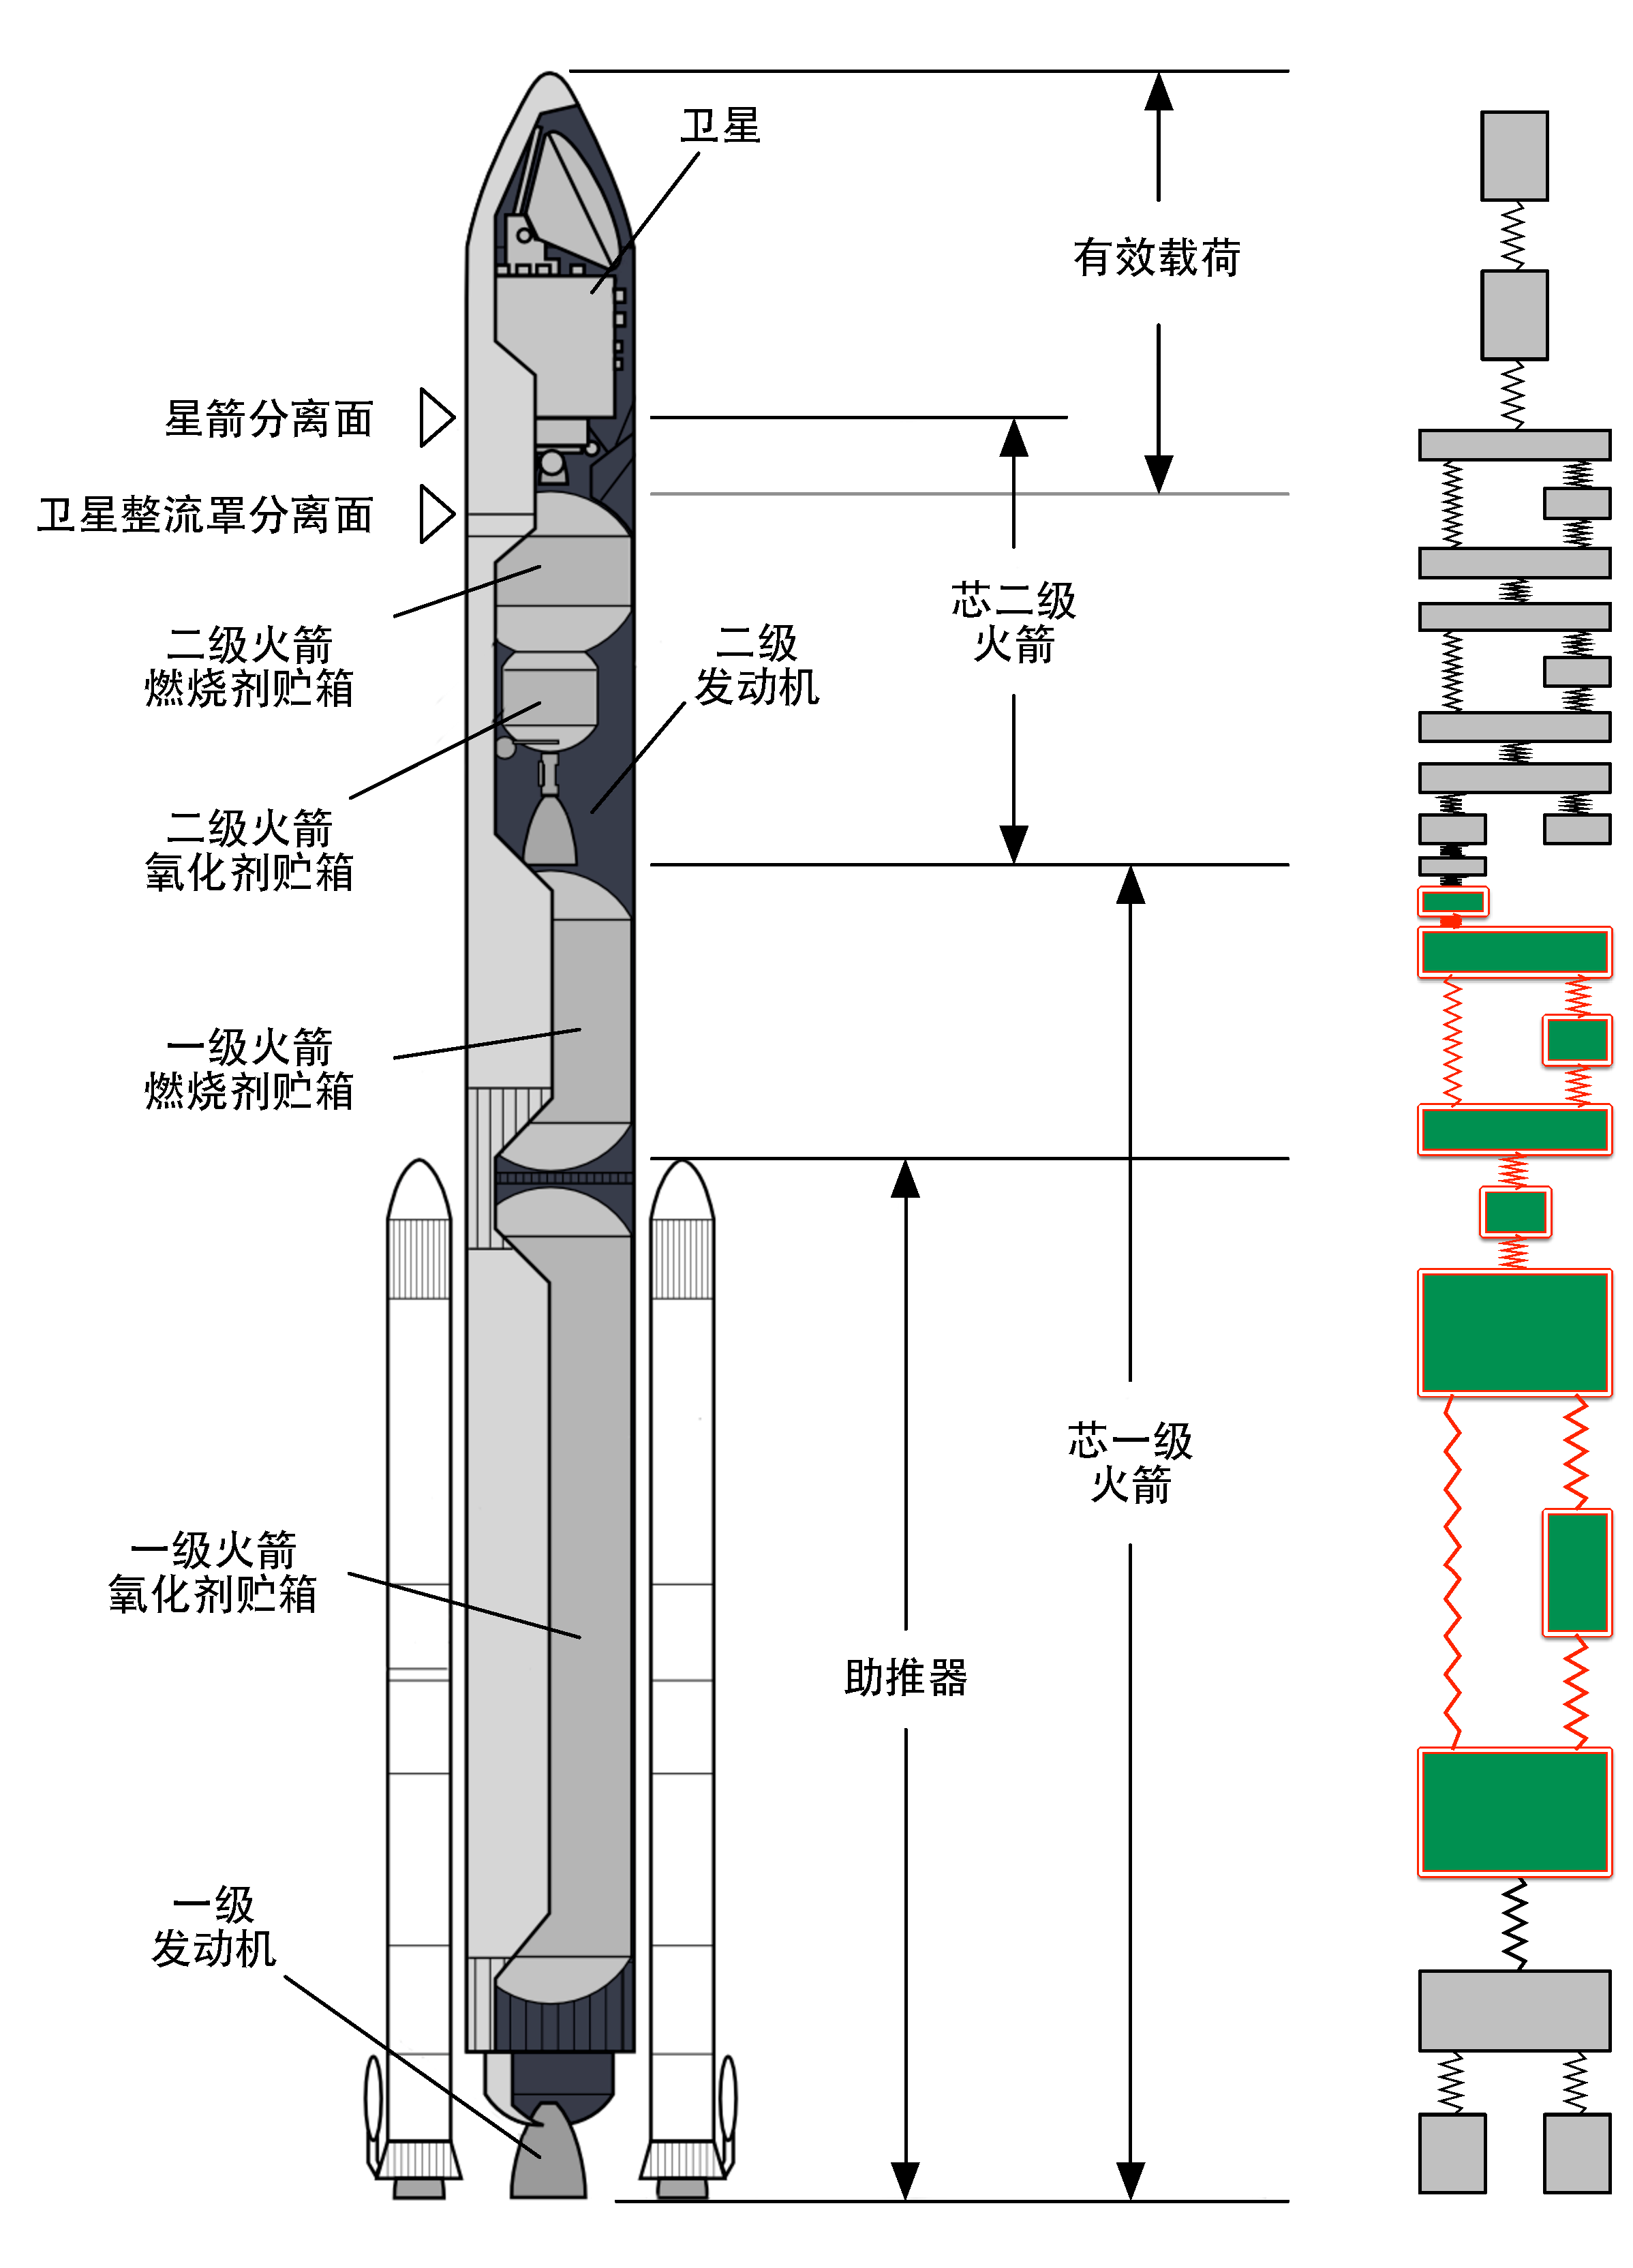
\includegraphics[width=.95\linewidth]{Whole-Rocket-Model}
  }
  \caption{液体火箭全箭集中质量模型}\label{Whole-Rocket-Model}
\end{figure}

\section{耦合系统稳定性分析方法}
传统的液体火箭POGO稳定性分析方法主要分为了矩阵法、单传法和临界阻尼法\cite{Wang-Qizheng:1999}等几类。从现代控制理论的角度出发\cite{Ogata:2009},这些方法从本质上看都是通过求解系统特征值来判断系统是否稳定:耦合系统特征值出现正实部则系统不稳定,若特征值实部全为负数则系统稳定。其中,矩阵法可分为闭环分析法和开环分析法,是传统POGO稳定性分析方法中最复杂、精度最高的。其余两种方法虽然计算过程较为简单,但由于计算结果精度较差,所以研究者们逐渐的将目光转向了更能满足目前工况计算要求的新型稳定性分析方法。本节将引入一种基于矩阵法的新型POGO稳定性快速求解方法。

根据公式\eqref{eq:Feedback-Force-Transfer}和\eqref{eq:Structure-Dynamic-Freq},可以把耦合系统的频域特征方程表示为:
\begin{equation}
  \label{eq:Coupled-System-Transfer-TMP}
  \left[s^2 \boldsymbol{M}_s+ s(\boldsymbol{C}_s+\boldsymbol{\dot{M}}_s)+ \boldsymbol{K}_s \right]\boldsymbol{X}_s(s)=\boldsymbol{F}_s(s)+ \boldsymbol{L}_{sp} \boldsymbol{R}_{pq}(s)\boldsymbol{\dot{X}}_q(s)
\end{equation}
若引入转换结构系统速度反馈节点位置的布尔矩阵,
\begin{displaymath}
  \boldsymbol{x}_q(t)=
  \left[ \begin{matrix}
      {x}_T(t) & {x}_{L1}^{(5)}(t)
    \end{matrix} \right]^{\ut}=
  \boldsymbol{L}_{qs} \boldsymbol{x}_s(t)
\end{displaymath}
可将公式\eqref{eq:Coupled-System-Transfer-TMP}改写为:
\begin{equation}
  \label{eq:Coupled-System-Transfer}
  \left[s^2 \boldsymbol{M}_s+ s\left(\boldsymbol{C}_s+\boldsymbol{\dot{M}}_s
    -\boldsymbol{L}_{sp} \boldsymbol{R}_{pq}(s)\boldsymbol{L}_{qs}\right)+ \boldsymbol{K}_s \right]\boldsymbol{X}_s(s)=\boldsymbol{F}_s(s)
\end{equation}
耦合系统稳定的准则是如下代数方程根的实部均不大于零:
\begin{equation}
  \label{eq:Coupled-Transfer-Det}
  \Psi (s) \triangleq \det
  \left[s^2 \boldsymbol{M}_s+ s\left(\boldsymbol{C}_s+\boldsymbol{\dot{M}}_s
    -\boldsymbol{L}_{sp} \boldsymbol{R}_{pq}(s)\boldsymbol{L}_{qs}\right)+ \boldsymbol{K}_s \right]\boldsymbol{X}_s(s)=0
\end{equation}

\subsection{反馈力传递函数的有理分式拟合方法}
从公式\eqref{eq:Coupled-Transfer-Det}的形式可以看出,耦合系统特征值问题的求解难点主要缘于阻抗函数$\boldsymbol{R}_{pq}(s)$的形式较为复杂。所以本节主要研究如何将其进行合理的等效变换,将包含了诸如双曲函数形式的管路系统反馈力传递函数转化为便于与液体火箭结构系统进行耦合分析的有理分式形式。

如果只考虑阻抗矩阵$\boldsymbol{R}_{pq}(s)$的单个元素,可以利用有理分式将此单输入单输出(SISO)传递函数在频域拟合为如下标准形式\cite{Gustavsen:1999, Zeng:2006}:
\begin{equation}
  \label{eq:Standard-SISO-Freq}
  T(\jmath\omega)=\jmath\omega M_0+ D_0+ \sum_{k=1}^{n}\frac{C_k}{\jmath\omega-A_k}+ \sum_{k=1}^{n}\frac{\bar{C}_k}{\jmath\omega- \bar{A}_k}+ \sum_{j=1}^{m} \frac{B_j}{\jmath\omega -R_j}
\end{equation}

其中$\jmath=\sqrt{-1}$,$A_k, R_j$为已知的极点,$M_0, D_0, C_k, B_j$为待定系数,符号$\bar{}$表示对应变量的共轭。值得注意的是,此处考虑了有理分式中包含成对出现的共轭极点、纯实数极点、直流分量和一次项的广义情况,实际拟合过程可能只需要保留其中的部分项。

根据离散的传递函数数据,可以在$n_f$个频率点上建立如下方程:
\begin{equation}
  \label{eq:Discrete-Standard-Transfer}
  T(\jmath\omega_f)=\jmath\omega_f M_0+ D_0+ \sum_{k=1}^{n}\frac{C_k}{\jmath\omega_f-A_k}+ \sum_{k=1}^{n}\frac{\bar{C}_k}{\jmath\omega_f- \bar{A}_k}+ \sum_{j=1}^{m} \frac{B_j}{\jmath\omega_f -R_j}
\end{equation}
记
\begin{align}
   & \boldsymbol{m}_1(\omega_f)=\left[ \begin{matrix}
      \jmath\omega_f & 1
    \end{matrix} \right] \nonumber \\
   & \boldsymbol{m}_2(\omega_f)=\left[ \begin{matrix}
      \displaystyle{\frac{1}{\jmath \omega_f-A_1}} & \cdots & \displaystyle{\frac{1}{\jmath \omega_f-A_n}} \\
    \end{matrix} \right] \nonumber \\
   & \boldsymbol{m}_3(\omega_f)=\left[ \begin{matrix}
      \displaystyle{\frac{1}{\jmath \omega_f-\bar{A}_1}} & \cdots & \displaystyle{\frac{1}{\jmath \omega_f-\bar{A}_n}} \\
    \end{matrix} \right]           \\
   & \boldsymbol{m}_4(\omega_f)=\left[ \begin{matrix}
      \displaystyle{\frac{1}{\jmath \omega_f-R_1}} & \cdots & \displaystyle{\frac{1}{\jmath \omega_f-R_m}} \\
    \end{matrix} \right] \nonumber \\
   & \boldsymbol{C}=\left[ \begin{matrix}
      C_1 & \cdots & C_n
    \end{matrix} \right]^{\ut} \nonumber       \\
   & \boldsymbol{B}=\left[ \begin{matrix}
      B_1 & \cdots & B_m
    \end{matrix} \right]^{\ut} \nonumber
\end{align}
可以将公式\eqref{eq:Discrete-Standard-Transfer}改写为:
\begin{equation}
  T(\jmath \omega_f)=\boldsymbol{m}_1(\omega_f)\left[
    \begin{matrix}
      M_0 \\
      D_0 \\
    \end{matrix} \right] + \boldsymbol{m}_2(\omega_f)\boldsymbol{C} + \boldsymbol{m}_3\boldsymbol{\bar{C}} +\boldsymbol{m}_4(\omega_f)\boldsymbol{B}
\end{equation}
将上式进行实部和虚部分离,方程变为
\begin{equation}
  \label{eq:SISO-Least-Square}
  \left[ \begin{matrix}
      T'(\omega_f)  \\
      T''(\omega_f) \\
    \end{matrix} \right]=\left[ \begin{matrix}
      \boldsymbol{m}'_1(\omega_f)                                & \boldsymbol{m}''_1(\omega_f)                               \\
      \boldsymbol{m}'_2(\omega_f)+ \boldsymbol{m}'_3(\omega_f)   & \boldsymbol{m}''_2(\omega_f)+ \boldsymbol{m}''_3(\omega_f) \\
      \boldsymbol{m}''_3(\omega_f)- \boldsymbol{m}''_2(\omega_f) & \boldsymbol{m}'_2(\omega_f)-\boldsymbol{m}'_3(\omega_f)    \\
      \boldsymbol{m}'_4(\omega_f)                                & \boldsymbol{m}''_4(\omega_f)                               \\
      -\boldsymbol{m}''_4(\omega_f)                              & \boldsymbol{m}'_4(\omega_f)
    \end{matrix} \right]^{\ut} \left[ \begin{matrix}
      M_0              \\
      D_0              \\
      \boldsymbol{C}'  \\
      \boldsymbol{C}'' \\
      \boldsymbol{B}'  \\
      \boldsymbol{B}'' \\
    \end{matrix} \right]
\end{equation}
其中,复数变量的记号约定如下:
\begin{equation}
  \Re(T)=T',\quad\Im(T)=T''
\end{equation}
利用最小二乘法\cite{Bjorck:1996},可以根据公式\eqref{eq:SISO-Least-Square}求解出有理分式\eqref{eq:Standard-SISO-Freq}中的各项待定系数。此外,如果发现拟合结果在某些重要频率范围内的精度达不到标的要求,还可以利用加权的最小二乘法\cite{Strutz:2011}对求解过程进行适当优化。

对于POGO研究中所涉及到的多输入多输出(MIMO)系统,可以利用上述方法对于阻抗矩阵$\boldsymbol{R}_{pq}(s)$中的各个分量进行分别拟合。值得注意的是,根据通过理论推导可以得知:管路系统反馈力传递矩阵中各个分量的极点是相同的,所以在对传递函数进行最小二乘法拟合之前,只需选其任意一个分量进行极点探测即可。如果在极点探测的过程中出现了由于数值误差或者拟合精度设置不统一等因素导致的极点不一致情况,工程上也可以将分别拟合得到的极点进行平均化处理。至于有理多项式拟合应采用多少极点,可以先解析的绘制出阻抗矩阵$\boldsymbol{R}_{pq}(s)$各分量的传递函数图形,根据曲线峰值的数目进行多项式项数的预估,然后根据具体的拟合结果进行拟合迭代次数和极点个数等参数的微调,最终得出合理的拟合结果。

\begin{figure}[p]
  \centering
  %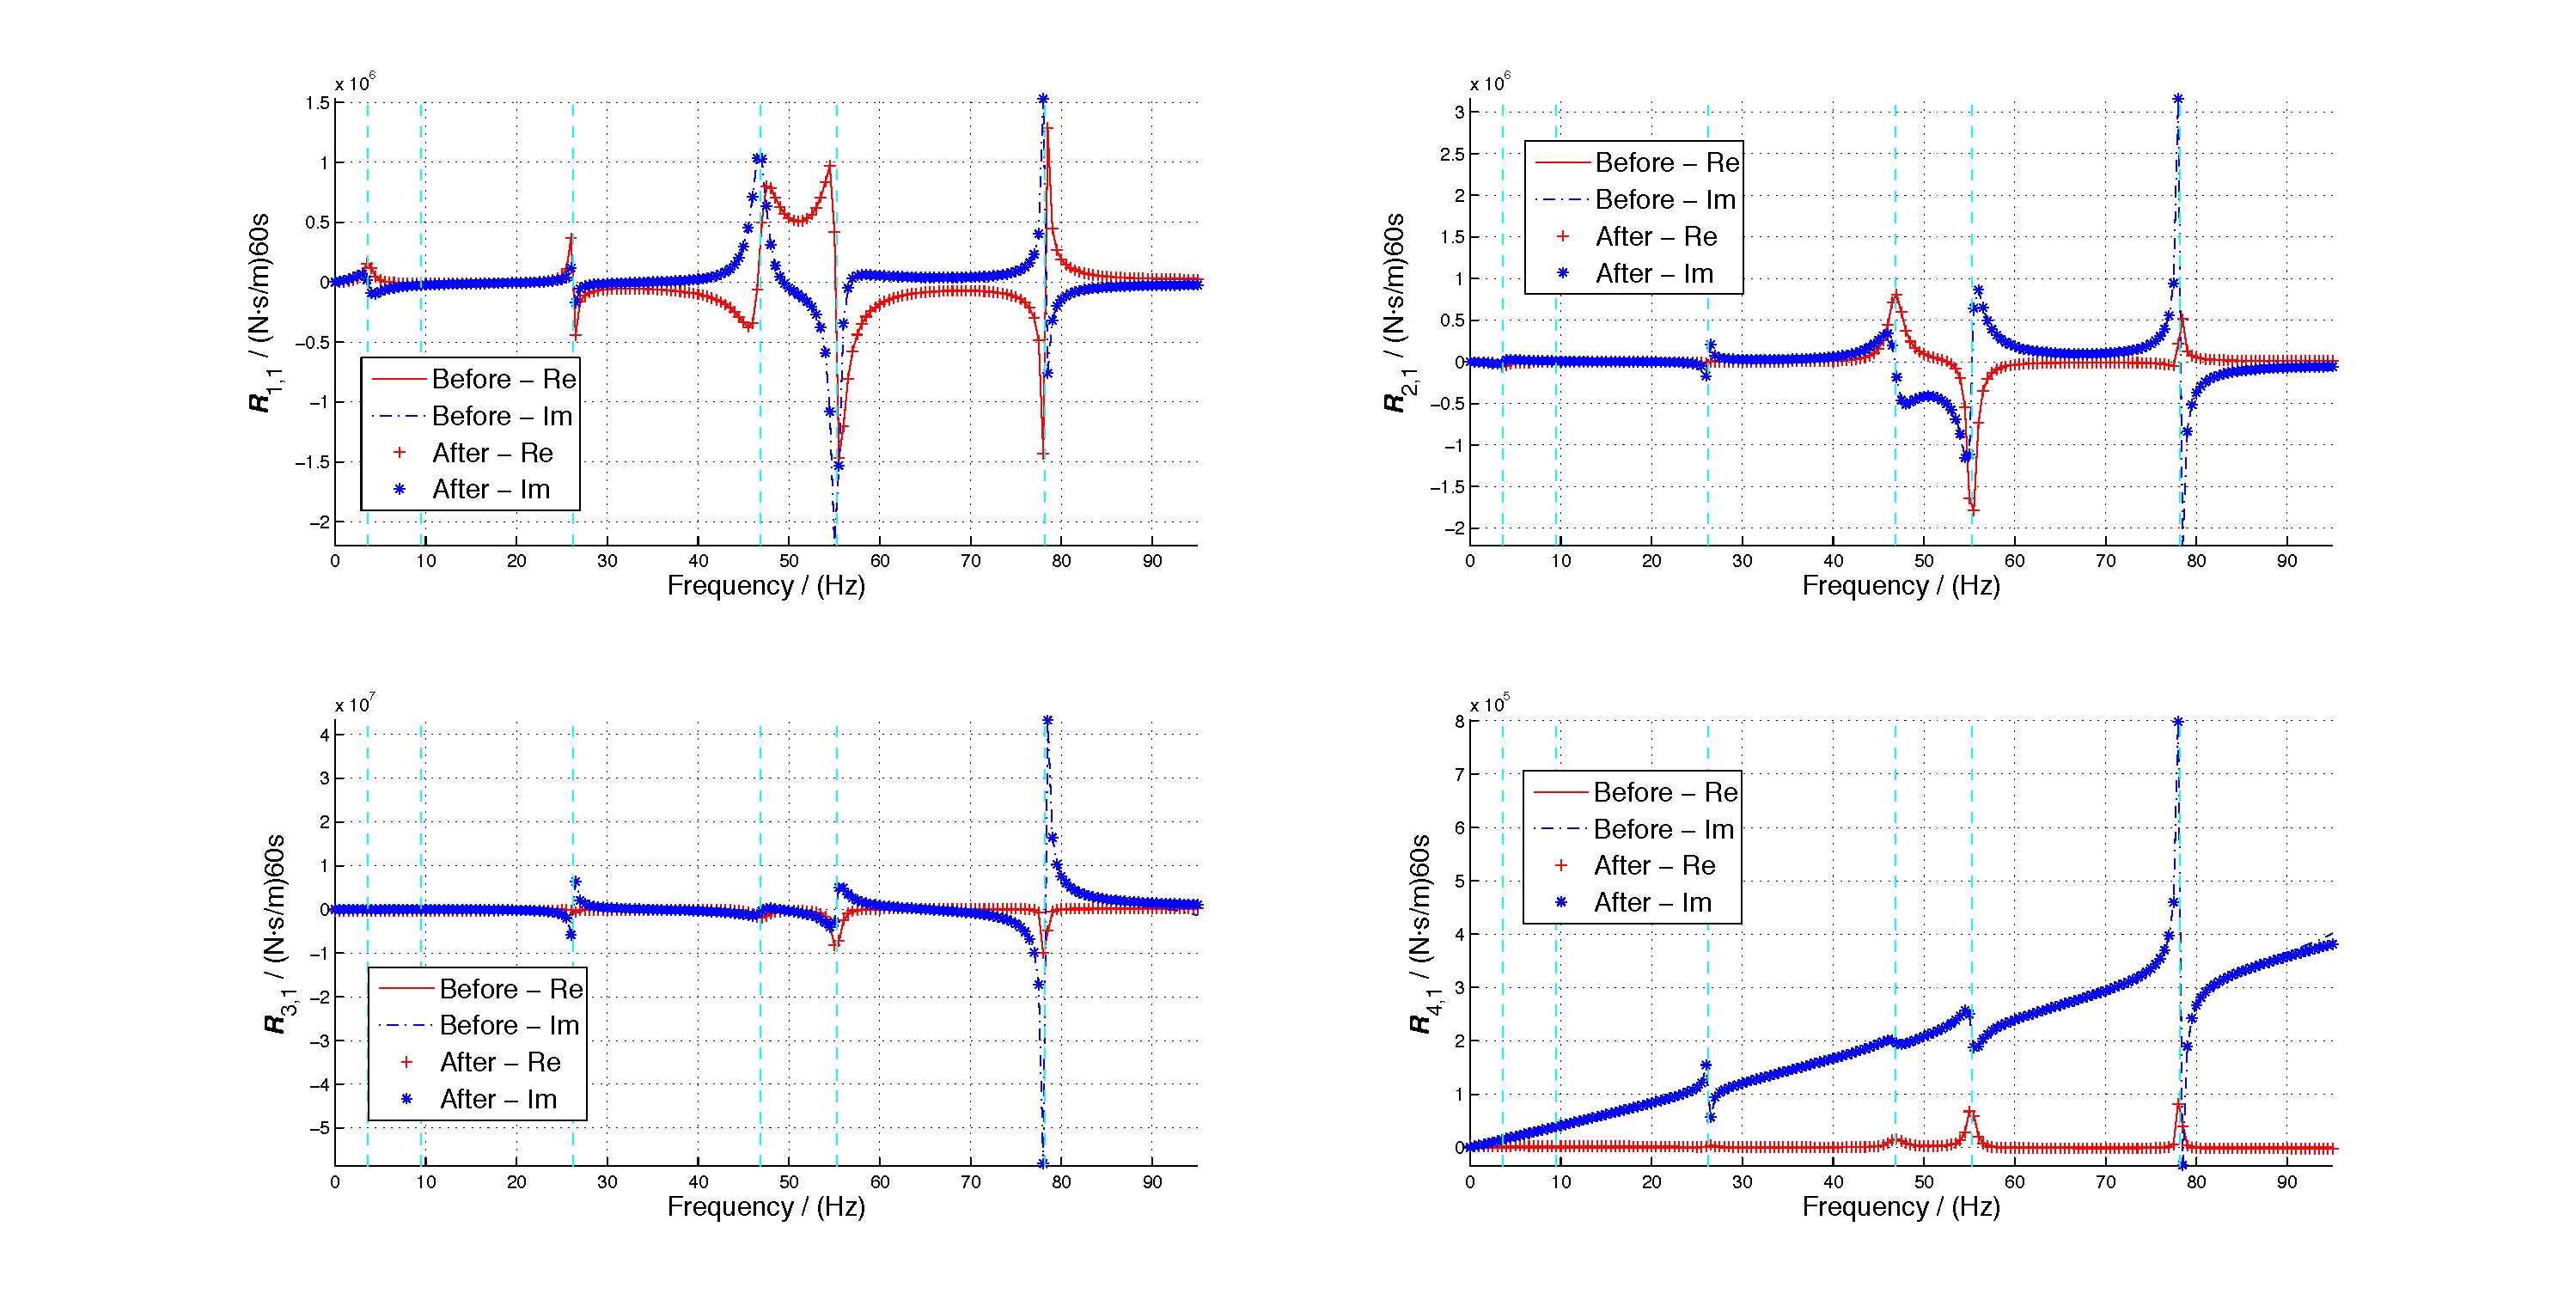
\includegraphics[trim={4.5cm 0cm 4.5cm 0cm}, clip=true, width=\linewidth]{Fitted-Transfer-01.pdf}
  \caption{管路系统反馈力有理分式拟合前后对比曲线(a):$\boldsymbol{R}_{11}-\boldsymbol{R}_{41}$}
  \label{Rational-Fitted-VS-01}
  \vspace{1.2em}
  %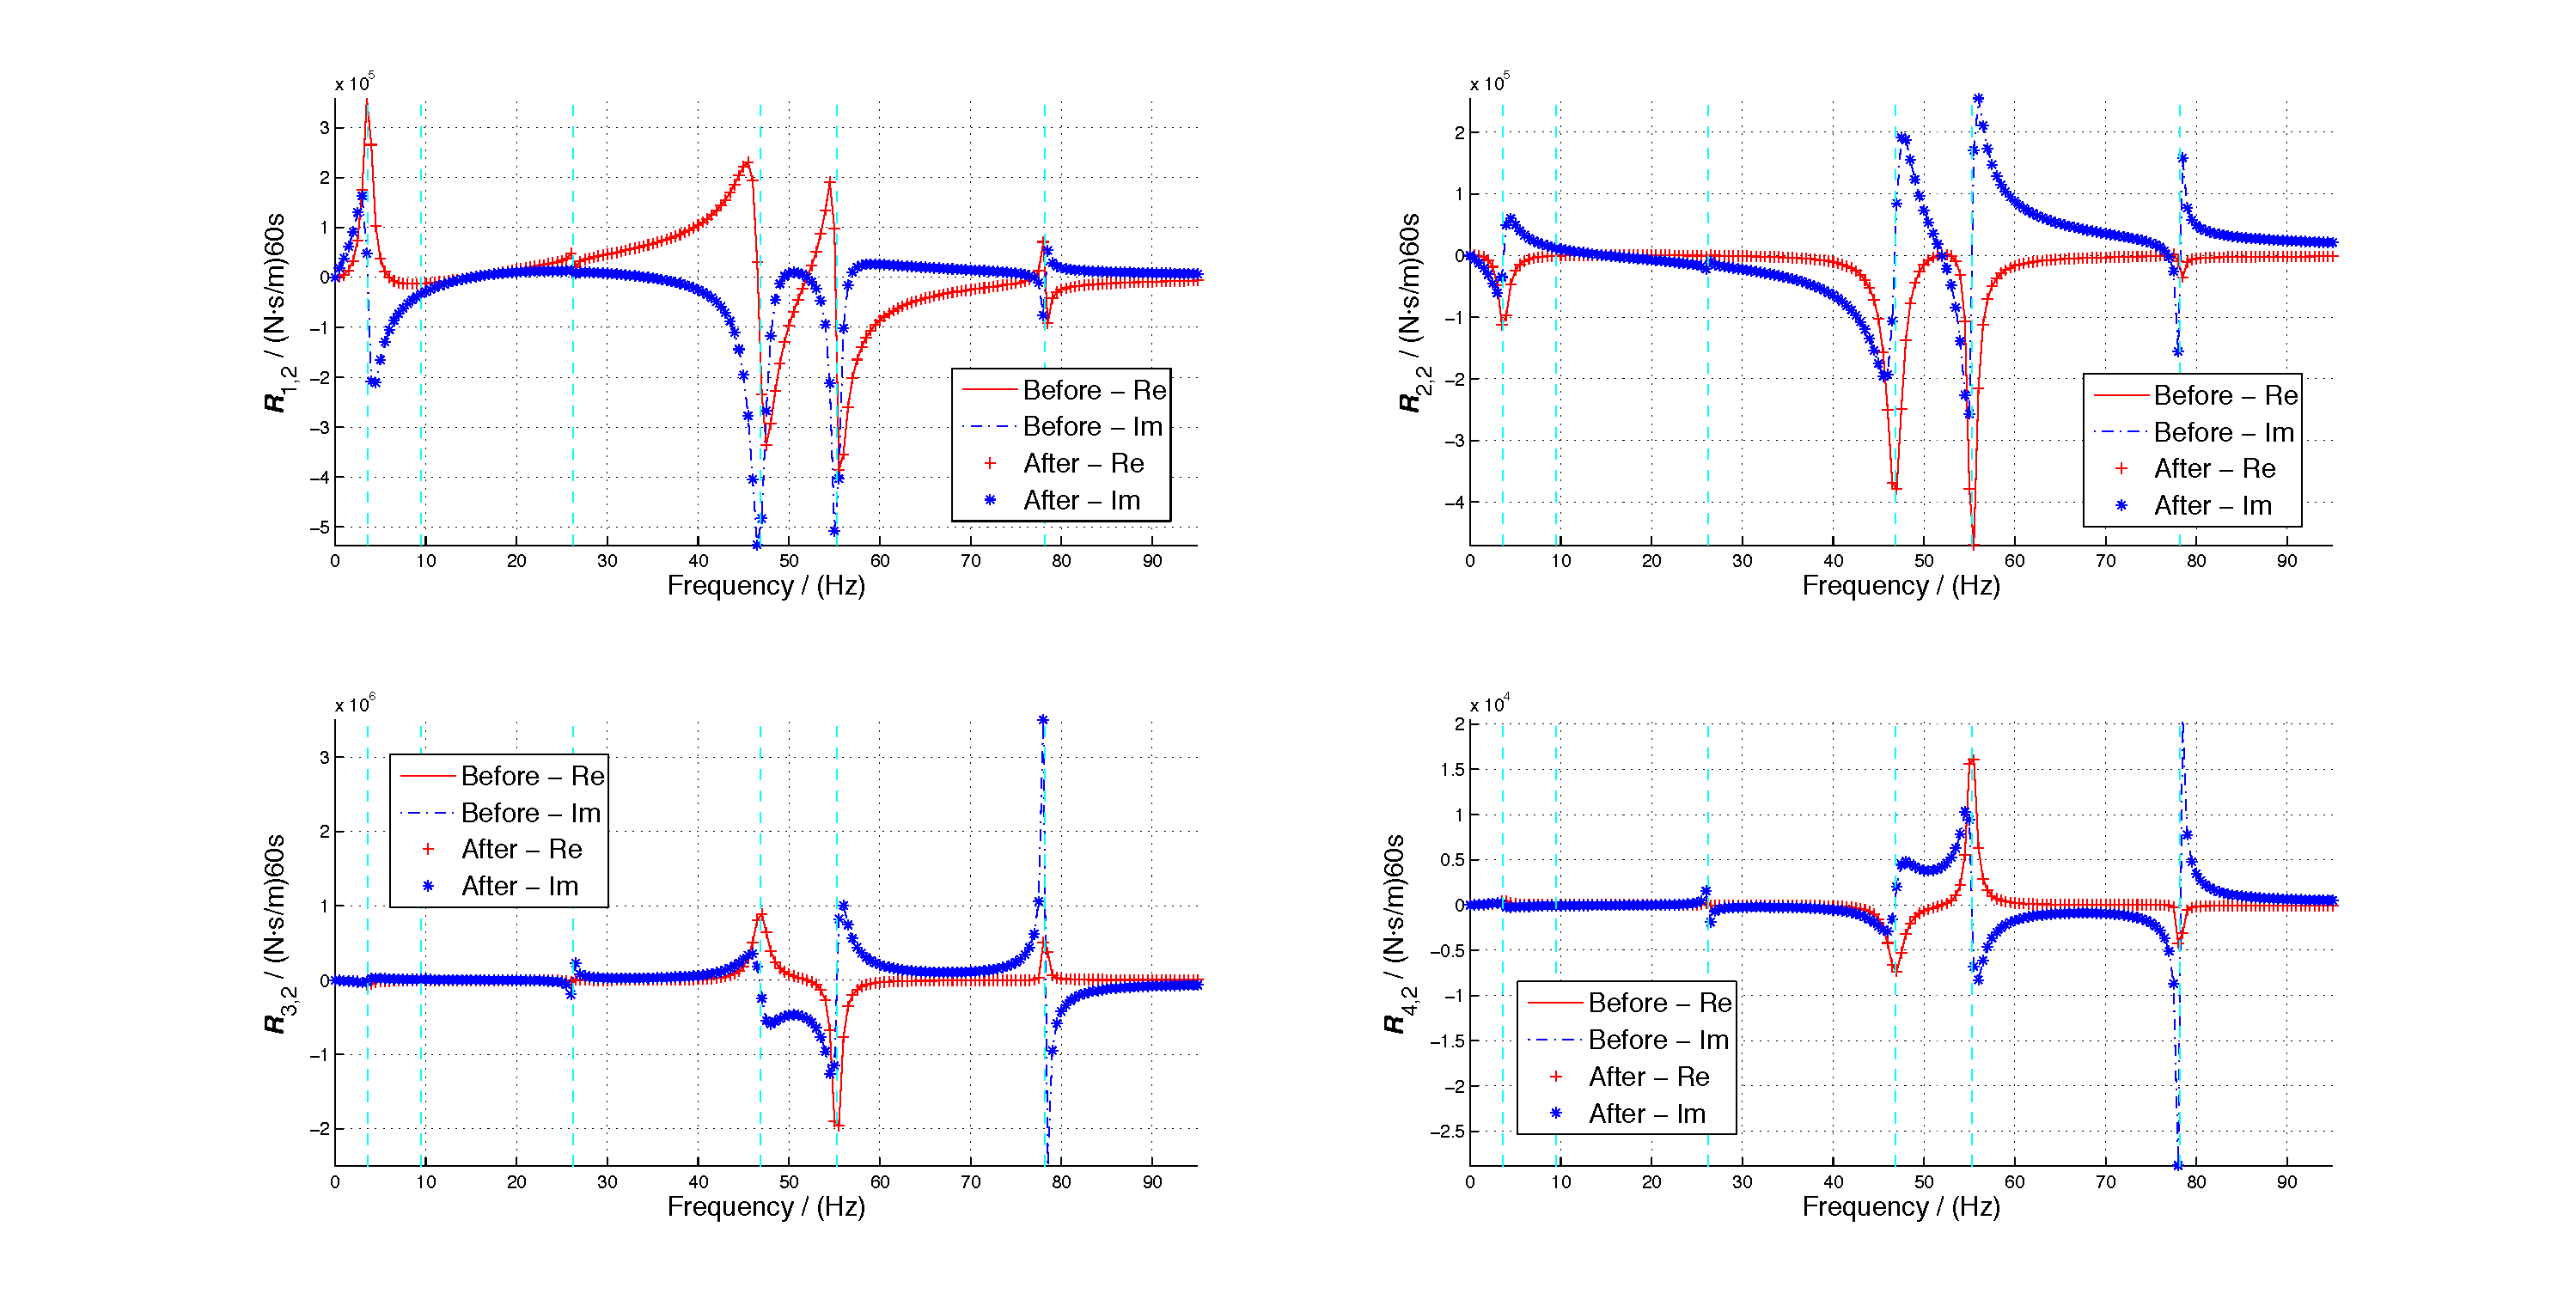
\includegraphics[trim={4.5cm 0cm 4.5cm 0cm}, clip=true, width=\linewidth]{Fitted-Transfer-02.pdf}
  \caption{管路系统反馈力有理分式拟合前后对比曲线(b):$\boldsymbol{R}_{12}-\boldsymbol{R}_{42}$}
  \label{Rational-Fitted-VS-02}
\end{figure}

至此,可以将推进系统作用到结构上的反馈力将表示为:
\begin{equation}
  \label{eq:Rational-Feedback-Force}
  \boldsymbol{F}_p(s)= \boldsymbol{R}_{pq}(s)\boldsymbol{\dot{X}}_q(s)
  =\left[ s\boldsymbol{M}_{pq}+ \boldsymbol{D}_{pq}+ \sum_{k=1}^n
    \left( \frac{\boldsymbol{C}_{pq}^{(k)}}{s-{A}_k} +
    \frac{\bar{\boldsymbol{C}}_{pq}^{(k)}}{s-\bar{A}_k}  \right)
    \right] \boldsymbol{\dot{X}}_q(s)
\end{equation}
其中$\boldsymbol{M}_{pq}, \boldsymbol{D}_{pq}$为实矩阵,${A}_k$为成对的共轭极点,$\boldsymbol{C}_{pq}^{(k)}$为成对的共轭矩阵,$p,q$分别表示阻抗矩阵的行数和列数,既管路系统反馈力和结构系统速度反馈节点的个数。在通常情况下,由于振动分析很少关注传递函数中包含纯实极点的情况,所以在拟合反馈力传递函数的时候并没有添加$R_j$项。

\subsection{反馈力传递矩阵的类结构化建模}
经过上节有理分式的拟合过程,管路系统反馈力传递函数已经被表示为了形如公式\eqref{eq:Rational-Feedback-Force}的较为简单形式。接下来,考虑对其进行进一步等效变换,通过引入辅助变量将有理分式转化为与结构振动方程相似的二阶常微分方程形式,便于进行下一步的耦合系统快速特征值求解。为此,考察$\boldsymbol{R}_{pq}(s)$其中一对共轭项:
\begin{equation}
  \label{eq:Feedback-Force-Original}
  \boldsymbol{F}_p^{(k)}(s)=\left( \frac{\boldsymbol{C}_{pq}^{(k)}}{s-A_k}+ \frac{\bar{\boldsymbol{C}}_{pq}^{(k)}}{s-\bar{A}_k} \right) \dot{\boldsymbol{X}_q}(s)
\end{equation}
对矩阵$\boldsymbol{C}_{pq}^{(k)}$做奇异值分解\cite{Golub:1996}
\begin{equation}
  \label{eq:QR-Dissect}
  \boldsymbol{C}_{pq}^{(k)}=\boldsymbol{U}_{pp}^{(k)}\boldsymbol{S}_{pq}^{(k)}{\boldsymbol{V}_{qq}^{(k)}}^{*}
\end{equation}
此处${}^*$表示矩阵的共轭转置,$\boldsymbol{S}_{pq}^{(k)}$形式如下
\begin{equation}
  \label{eq:SVD-Rank-Analysis}
  \boldsymbol{S}_{pq}^{(k)}=\left[ \begin{matrix}
      \boldsymbol{S}_{r_kr_k}^{(k)} & \boldsymbol{0}_{r_k(q-r_k)}     \\
      \boldsymbol{0}_{(p-r_k)}      & \boldsymbol{0}_{(p-r_k)(q-r_k)} \\
    \end{matrix} \right]
\end{equation}
$r_k$为矩阵$\boldsymbol{C}_{pq}^{(k)}$的秩,$\boldsymbol{S}_{r_kr_k}^{(k)}$为非奇异实对角矩阵,$\boldsymbol{U}_{pp}^{(k)}, \boldsymbol{V}_{qq}^{(k)}$为复矩阵,满足:
\begin{equation}
  {\boldsymbol{U}_{pp}^{(k)}}^*\boldsymbol{U}_{pp}^{(k)}=\boldsymbol{I}_{pp},
  {\boldsymbol{V}_{qq}^{(k)}}^*\boldsymbol{V}_{qq}^{(k)}=\boldsymbol{I}_{qq}
\end{equation}
分别从矩阵$\boldsymbol{U}_{pp}^{(k)}, \boldsymbol{V}_{qq}^{(k)}$中取出前$r_k$列,构成列满秩矩阵$\boldsymbol{U}_{pr_k}^{(k)}, \boldsymbol{V}_{qr_k}^{(k)}$,将公式\eqref{eq:QR-Dissect}表示成
\begin{equation}
  \boldsymbol{C}_{pq}^{(k)}=\boldsymbol{U}_{pr_k}^{(k)}\boldsymbol{S}_{r_kr_k}^{(k)}{\boldsymbol{V}_{qr_k}^{(k)}}^{*}
\end{equation}
这样,可以将推进系统反馈力$\boldsymbol{F}_p^{(k)}(s)$改写为:
\begin{equation}
  \label{eq:Single-SVD-Feedback-Force}
  \boldsymbol{F}_p^{(k)}(s)=\left( \frac{
  \boldsymbol{U}_{pr_k}^{(k)}\boldsymbol{S}_{r_kr_k}^{(k)}{\boldsymbol{V}_{qr_k}^{(k)}}^{*}
  }{s-A_k}+ \frac{
  \boldsymbol{\bar{U}}_{pr_k}^{(k)}\boldsymbol{S}_{r_kr_k}^{(k)}{\boldsymbol{\bar{V}}}{{}_{qr_k}^{(k)}}^{*}
  }{s-\bar{A}_k} \right) \dot{\boldsymbol{X}_q}(s)
\end{equation}

\noindent 定义两组关于时间的实函数$\boldsymbol{y}_{r_k}^{\prime(k)}(t), \boldsymbol{y}_{r_k}^{\prime\prime(k)}(t)$,在时域满足微分方程
\begin{equation}
  \label{eq:Extra-Variable-ODE}
  \left\{
  \begin{aligned}
    \dot{\boldsymbol{y}}_{r_k}^{\prime(k)}(t)- A'_k\boldsymbol{y}_{r_k}^{\prime(k)}(t)+A''_k\boldsymbol{y}_{r_k}^{\prime\prime(k)}(t)       & = {\boldsymbol{V}_{qr_k}^{\prime(k)}}^{\ut} \boldsymbol{x}_{q}(t)        \\
    \dot{\boldsymbol{y}}_{r_k}^{\prime\prime(k)}(t)-A''_k \boldsymbol{y}_{r_k}^{\prime(k)}(t)-A'_k\boldsymbol{y}_{r_k}^{\prime\prime(k)}(t) & = -{\boldsymbol{V}_{qr_k}^{\prime\prime(k)}}^{\ut} \boldsymbol{x}_{q}(t)
  \end{aligned} \right.
\end{equation}
其中,复数变量的记号约定同上节:$A'_k=\Re(A_k),A''_k=\Im(A_k)$,复矩阵在写法上亦采用相同规范
\begin{displaymath}
  \boldsymbol{V}_{qr_k}^{\prime(k)}=\Re(\boldsymbol{V}_{qr_k}^{(k)}), \boldsymbol{V}_{qr_k}^{\prime\prime(k)}=\Im(\boldsymbol{V}_{qr_k}^{(k)})
\end{displaymath}
$\boldsymbol{x}_q(t)$是$\boldsymbol{X}_q(s)$的Laplace逆变换:
\begin{displaymath}
  \boldsymbol{x}_q(t)=\Lacelap{\boldsymbol{X}_q(s)}
\end{displaymath}
将公式\eqref{eq:Extra-Variable-ODE}进行Laplace变换,
\begin{equation}
  \label{eq:Extra-Variable-Laplace}
  \left\{
  \begin{aligned}
    (s-A'_k)\boldsymbol{Y}_{r_k}^{\prime(k)}(s)+ A''_k\boldsymbol{Y}_{r_k}^{\prime\prime(k)}(s)  & ={\boldsymbol{V}_{qr_k}^{\prime(k)}}^{\ut}\boldsymbol{X}_q(s)         \\
    -A''_k\boldsymbol{Y}_{r_k}^{\prime(k)}(s)+ (s-A'_k)\boldsymbol{Y}_{r_k}^{\prime\prime(k)}(s) & = -{\boldsymbol{V}_{qr_k}^{\prime\prime(k)}}^{\ut}\boldsymbol{X}_q(s)
  \end{aligned} \right.
\end{equation}
其中
\begin{align}
  \boldsymbol{Y}_{r_k}^{\prime(k)}(s)       & =\Laplace{\boldsymbol{y}_{r_k}^{\prime(k)}(t)} \nonumber       \\
  \boldsymbol{Y}_{r_k}^{\prime\prime(k)}(s) & =\Laplace{\boldsymbol{y}_{r_k}^{\prime\prime(k)}(t)} \nonumber \\
  \boldsymbol{X}_q(s)                       & = \Laplace{\boldsymbol{x}_q(t)} \nonumber
\end{align}
可以验证,满足方程\eqref{eq:Extra-Variable-Laplace}的函数$\boldsymbol{Y}_{r_k}^{\prime(k)}, \boldsymbol{Y}_{r_k}^{\prime\prime(k)}$必然满足:
\begin{subequations}
  \label{eq:Extra-Variable-Laplace-Displacement}
  \begin{align}
    {\displaystyle\frac{{\boldsymbol{V}_{qr_k}^{(k)}}^{*}}{(s-A_k)}} \boldsymbol{X}_q(s)               & = \boldsymbol{Y}_{r_k}^{\prime(k)}(s)+ \jmath\boldsymbol{Y}_{r_k}^{\prime\prime(k)}(s)  \label{eq:Extra-Variable-Laplace-Displacement-01} \\
    {\displaystyle\frac{\boldsymbol{\bar{V}}{{}_{qr_k}^{(k)}}^{*}}{(s-\bar{A}_k)}} \boldsymbol{X}_q(s) & = \boldsymbol{Y}_{r_k}^{\prime(k)}(s)- \jmath\boldsymbol{Y}_{r_k}^{\prime\prime(k)}(s)  \label{eq:Extra-Variable-Laplace-Displacement-02}
  \end{align}
\end{subequations}
将公式\eqref{eq:Extra-Variable-Laplace-Displacement}带入\eqref{eq:Single-SVD-Feedback-Force},$\boldsymbol{F}_p^{(k)}(s)$可以写为:
\begin{equation}
  \label{eq:Feedback-Single-Force-Extra-Variable}
  \boldsymbol{F}_p^{(k)}(s)=2\left[ \boldsymbol{U}_{pr_k}^{\prime(k)}\boldsymbol{S}_{r_kr_k}^{(k)} \dot{\boldsymbol{Y}}_{r_k}^{\prime(k)}(s)-
    \boldsymbol{U}_{pr_k}^{\prime\prime(k)}\boldsymbol{S}_{r_kr_k}^{(k)} \dot{\boldsymbol{Y}}_{r_k}^{\prime\prime(k)}(s)
    \right]
\end{equation}
观察方程\eqref{eq:Extra-Variable-Laplace-Displacement-01},可以看出
\begin{equation}
  \label{eq:Extra-Variable-Displacement-Final}
  \boldsymbol{Y}_{r_k}^{\prime\prime(k)}(s)= {\displaystyle\frac{{\boldsymbol{V}_{qr_k}^{\prime(k)}}^{\ut} \boldsymbol{X}_q(s)-(s-A'_k)\boldsymbol{Y}_{r_k}^{\prime(k)}(s)}{A''_k}}
\end{equation}
若将\eqref{eq:Extra-Variable-Displacement-Final}分别带入公式\eqref{eq:Feedback-Single-Force-Extra-Variable}和\eqref{eq:Extra-Variable-Laplace-Displacement-02},可以导出
\begin{equation}
  \label{eq:Feedback-Force-Final}
  \left\{
  \begin{aligned}
    s\boldsymbol{D}_{pq}^{(k)}\boldsymbol{X}_{q}(s)+ s^2\boldsymbol{M}_{pr_k}^{(k)}\boldsymbol{Y}_{r_k}^{\prime(k)}(s)+ s\boldsymbol{D}_{pr_k}^{(k)}\boldsymbol{Y}_{r_k}^{\prime(k)}(s) & = \boldsymbol{F}_{p}^{(k)}(s) \\
    s^{2}\boldsymbol{Y}_{r_k}^{\prime(k)}(s)-s{\boldsymbol{V}_{qr_k}^{\prime(k)}}^{\ut} \boldsymbol{X}_{q}(s)- 2sA'_k\boldsymbol{Y}_{r_k}^{\prime(k)}(s)                                                                \\
    \qquad {} + \boldsymbol{K}_{r_kq}^{(k)}\boldsymbol{X}_{q}(s)+ ({A'_k}^2+{A''_k}^{2})\boldsymbol{Y}_{r_k}^{\prime(k)}(s)                                                             & =  \boldsymbol{0}_{r_k}
  \end{aligned} \right.
\end{equation}
其中,
\begin{displaymath}
  \begin{aligned}
    \boldsymbol{M}_{pr_k}^{(k)}=\frac{2}{A''_k} \boldsymbol{U}_{pr_k}^{\prime\prime(k)} \boldsymbol{S}_{r_kr_k}^{(k)}                                          & , \; \boldsymbol{K}_{r_kq}^{(k)}= {A'_k} {\boldsymbol{V}_{qr_k}^{\prime(k)}}^{\ut}- {A''_k}{\boldsymbol{V}_{qr_k}^{\prime\prime(k)}}^{\ut}                             \\
    \boldsymbol{D}_{pq}^{(k)}=-\frac{2}{A''_k} \boldsymbol{U}_{pr_k}^{\prime\prime(k)} \boldsymbol{S}_{r_kr_k}^{(k)} {\boldsymbol{V}_{qr_k}^{\prime(k)}}^{\ut} & , \; \boldsymbol{D}_{pr_k}^{(k)}=\frac{2}{A''_k}(A''_{k}\boldsymbol{U}_{pr_k}^{\prime(k)}- {A'_k}\boldsymbol{U}_{pr_k}^{\prime\prime(k)})\boldsymbol{S}_{r_kr_k}^{(k)}
  \end{aligned}
\end{displaymath}
考察公式\eqref{eq:Feedback-Force-Final},若将方程组中的变量$\boldsymbol{Y}_{r_k}^{\prime(k)}(s)$消去,将得到与公式\eqref{eq:Feedback-Force-Original}形式相同的推进系统反馈力$\boldsymbol{F}_p^{(k)}(s)$与结构反馈速度$\dot{\boldsymbol{X}}_q(s)$传递关系,因此方程\eqref{eq:Feedback-Force-Final}与\eqref{eq:Feedback-Force-Original}在数学上是等价的。

在实际操作过程当中,通常可以观察到公式\eqref{eq:SVD-Rank-Analysis}中$\boldsymbol{S}_{r_kr_k}^{(k)}$的元素存在如下规律:$\alpha_1\gg\alpha_n,\ n=2\dots r_k$\footnote{在SVD分解的过程中,按照常见的做法将奇异值由大而小排列}。
\begin{displaymath}
  \boldsymbol{S}_{r_kr_k}^{(k)}= \begin{bmatrix}
    \rule{2pt}{0ex}\alpha_1                                           &        & \text{\raisebox{-1.2ex}{\makebox[0pt][c]{\huge0}}} \\[0em]
                                                                      & \ddots &                                                    \\[0em]
    \text{\rule{1pt}{0ex}\raisebox{-0.4ex}{\makebox[0pt][c]{\huge0}}} &        & \alpha_{r_k}                                       \\[0em]
  \end{bmatrix}
\end{displaymath}
为了尽量减少辅助变量$\boldsymbol{Y}_{r_k}^{\prime(k)}$的个数\footnote{辅助变量的总数为:$\sum_{k=1}^n r_n$,既$\boldsymbol{S}_{r_kr_k}^{(k)}$非零奇异值数目之和},在不显著影响传递关系精度的情况下可以将除$\alpha_1$之外的奇异值置零。

利用方程\eqref{eq:Feedback-Force-Final},一般形式的管路系统反馈力传递函数\eqref{eq:Rational-Feedback-Force}最终可以等效成为:
\begin{equation}
  \label{eq:Final-Common-Feedback-SVD-Force}
  \left\{
  \begin{aligned}
     & ({s}^{2}{\boldsymbol{M}_{pq}}+s{\boldsymbol{C}_{pq}})\boldsymbol{X}_{q}(s)+({s}^{2}\boldsymbol{M}_{pr_T}+s{\boldsymbol{B}_{pr_T}})\boldsymbol{Y}_{r_T}(s)=\boldsymbol{F}_{p}(s)                            \\
     & (s\boldsymbol{V}_{r_Tq}+\boldsymbol{K}_{r_Tq})\boldsymbol{X}_{q}(s)+(s^2\boldsymbol{I}_{r_Tr_T}+s\boldsymbol{\Lambda}_{r_Tr_T} + \boldsymbol{\Omega}_{r_Tr_T})\boldsymbol{Y}_{r_T}(s)=\boldsymbol{0}_{r_T}
  \end{aligned} \right.
\end{equation}
其中
\begin{displaymath}
  \begin{aligned}
     & \boldsymbol{C}_{pq}=\boldsymbol{D}_{pq}+\sum_{k=1}^{n}{\boldsymbol{D}_{pq}^{(k)}} ,\
    \boldsymbol{M}_{pr_T}=\left[ \begin{matrix}
        \boldsymbol{M}_{pr_1}^{(1)} & \cdots & \boldsymbol{M}_{pr_n}^{(n)}
      \end{matrix} \right] ,\
    \boldsymbol{B}_{pr_T}=\left[ \begin{matrix}
        \boldsymbol{D}_{pr_1}^{(1)} & \cdots & \boldsymbol{D}_{pr_n}^{(n)}
      \end{matrix} \right]                         \\
     & \boldsymbol{K}_{r_Tq}=\left[ \begin{matrix}
        {\boldsymbol{K}_{r_1q}^{(1)}}^{\ut} \\
        \vdots                              \\
        {\boldsymbol{K}_{r_nq}^{(n)}}^{\ut}
      \end{matrix} \right], \
    \boldsymbol{V}_{r_Tq}=\left[ \begin{matrix}
        -{\boldsymbol{V}_{qr_1}^{\prime(1)}}^{\ut} \\
        \vdots                                     \\
        -{\boldsymbol{V}_{qr_n}^{\prime(n)}}^{\ut}
      \end{matrix} \right], \
    \boldsymbol{Y}_{r_T}(s)=\left[ \begin{matrix}
        \boldsymbol{Y}_{r_1}^{\prime(1)}(s) \\
        \vdots                              \\
        \boldsymbol{Y}_{r_n}^{\prime(n)}(s)
      \end{matrix} \right],\
    r_T= \sum_{k=1}^n r_n                                                                   \\
     & \boldsymbol{\Omega}_{r_Tr_T}=\operatorname{diag} \left(
    \begin{matrix}
        ({A}_{1}^{\prime 2}+{A}^{\prime\prime 2}_{1}) \boldsymbol{I}_{r_1} & \cdots & ({A}_{n}^{\prime 2}+{A}_{n}^{\prime\prime 2})\boldsymbol{I}_{r_n}
      \end{matrix}
    \right)                                                                                 \\
     & \boldsymbol{\Lambda}_{r_Tr_T}=\operatorname{diag}\left(
    \begin{matrix}
        -2A'_{1}\boldsymbol{I}_{r_1} & \cdots & -2{A'_{n}}\boldsymbol{I}_{r_n}
      \end{matrix}
    \right)
  \end{aligned}
\end{displaymath}

为了验证公式\eqref{eq:Final-Common-Feedback-SVD-Force}与原始管路系统反馈力传递函数\eqref{eq:Feedback-Force-Transfer}之间的等价性,图\ref{SVD-Fitted-VS-01}和\ref{SVD-Fitted-VS-02}仿照之前做法(同样为液体火箭升空后60s),给出了两种结果之间的对比曲线。可以看出,即使此处强制使得$\alpha_n=0,\ n=2\dots r_k$,既$\boldsymbol{C}_{pq}^{(k)}$秩为一,拟合后的反馈力阻抗曲线依然可以达到很高的精度\footnote{若对比曲线之间相差较大,可以采用最小二乘法对于$\alpha_1$关于原始采样数据进行修正}。

至此,若将经过类结构化处理的管路系统反馈力表达式\eqref{eq:Final-Common-Feedback-SVD-Force}代入结构系统有限元模型的运动方程\eqref{eq:Coupled-System-Transfer},最终可以得到Laplace域的耦合系统动力学方程:
\begin{equation}
  \label{eq:Final-Coupled-System-Laplace}
  \left\{
  \begin{aligned}
    (s^2\boldsymbol{M}_{ss}+ s\boldsymbol{C}_{ss}+ \boldsymbol{K}_{s}) \boldsymbol{X}_{s}(s)+(s^2\boldsymbol{M}_{sr_T}+s\boldsymbol{B}_{sr_T}) \boldsymbol{Y}_{r_T}(s)                    & =\boldsymbol{F}_{s}(s) \\
    (s\boldsymbol{V}_{r_Ts}+\boldsymbol{K}_{r_Ts})\boldsymbol{X}_{s}(s)+(s^2\boldsymbol{I}_{r_Tr_T}+s\boldsymbol{\Lambda}_{r_Tr_T}+\boldsymbol{\Omega}_{r_Tr_T})\boldsymbol{Y}_{r_{T}}(s) & =\boldsymbol{0}_{r_T}
  \end{aligned} \right.
\end{equation}
其中
\begin{displaymath}
  \begin{aligned}
     & \boldsymbol{M}_{ss}=\boldsymbol{M}_{s}-\boldsymbol{L}_{sp}\boldsymbol{M}_{pq}\boldsymbol{L}_{qs},\
    \boldsymbol{M}_{sr_T}=-\boldsymbol{L}_{sp}\boldsymbol{M}_{pr_T},\
    \boldsymbol{K}_{r_Ts}=\boldsymbol{K}_{r_Tq}\boldsymbol{L}_{qs}                                        \\
     & \boldsymbol{B}_{sr_{T}}=-\boldsymbol{L}_{sp}\boldsymbol{B}_{pr_T},\
    \boldsymbol{C}_{ss}=\boldsymbol{C}_{s}+\dot{\boldsymbol{M}}_s -\boldsymbol{L}_{sp}\boldsymbol{C}_{pq}\boldsymbol{L}_{qs},\
    \boldsymbol{V}_{r_Ts}=\boldsymbol{V}_{r_Tq}\boldsymbol{L}_{qs}
  \end{aligned}
\end{displaymath}
若将上式变换到时域,可以得到类似于常规结构系统的耦合系统动力学方程
\begin{equation}
  \label{eq:Final-Coupled-1D-Transfer}
  \boldsymbol{M}_c\ddot{\boldsymbol{x}}_c+\boldsymbol{C}_c\dot{\boldsymbol{x}}_c+\boldsymbol{K}_c\boldsymbol{x}_c=\boldsymbol{f}_c(t)
\end{equation}
其中
\begin{displaymath}
  \begin{aligned}
     & \boldsymbol{x}_{c}=\left[ \begin{matrix}
        \boldsymbol{x}_{s}   \\
        \boldsymbol{y}_{r_T} \\
      \end{matrix} \right],\
    \boldsymbol{f}_c(t)=\left[ \begin{matrix}
        \boldsymbol{f}_{s}(t) \\
        \boldsymbol{0}_{r_T}  \\
      \end{matrix} \right],\
    \boldsymbol{M}_{c}=\left[ \begin{matrix}
        \boldsymbol{M}_{ss}   & \boldsymbol{M}_{sr_T}   \\
        \boldsymbol{0}_{r_Ts} & \boldsymbol{I}_{r_Tr_T} \\
      \end{matrix} \right]      \\
     & \boldsymbol{C}_{c}=\left[ \begin{matrix}
        \boldsymbol{C}_{ss}   & \boldsymbol{B}_{sr_T}         \\
        \boldsymbol{V}_{r_Ts} & \boldsymbol{\Lambda}_{r_Tr_T}
      \end{matrix} \right],\
    \boldsymbol{K}_{c}=\left[ \begin{matrix}
        \boldsymbol{K}_{s}    & \boldsymbol{0}_{sr_T}        \\
        \boldsymbol{K}_{r_Ts} & \boldsymbol{\Omega}_{r_Tr_T} \\
      \end{matrix} \right]
  \end{aligned}
\end{displaymath}
方程\eqref{eq:Final-Coupled-1D-Transfer}的特征值可采用状态空间方法进行求解。令$\boldsymbol{y}_c=\dot{\boldsymbol{x}}_c,\ \boldsymbol{z}={[ {\boldsymbol{y}_c}^{\ut}\quad {\boldsymbol{x}_c}^{\ut} ]}^{\ut}$,可以将其改写为:
\begin{equation}
  \boldsymbol{A}\dot{\boldsymbol{z}}+ \boldsymbol{B}\boldsymbol{z}=\boldsymbol{f}(t)
\end{equation}
其中
\begin{displaymath}
  \boldsymbol{A}=\left[ \begin{matrix}
      \boldsymbol{0}     & \boldsymbol{M}_{c} \\
      \boldsymbol{M}_{c} & \boldsymbol{C}_{c} \\
    \end{matrix} \right],\
  \boldsymbol{B}=\left[ \begin{matrix}
      -\boldsymbol{M}_{c} & \boldsymbol{0}     \\
      \boldsymbol{0}      & \boldsymbol{K}_{c} \\
    \end{matrix} \right],\
  \boldsymbol{f}(t)=\left[ \begin{matrix}
      \boldsymbol{0}        \\
      \boldsymbol{f}_{c}(t) \\
    \end{matrix} \right]
\end{displaymath}
最后,耦合系统的特征值求解便可归结为矩阵特征值问题:
\begin{equation}
  \label{eq:Fast-Matrix-Eigen-Equation}
  \left( \lambda \boldsymbol{A}+ \boldsymbol{B} \right)\boldsymbol{\psi}_c=0
\end{equation}

\section{算例分析}
\label{sec:Lumped-Numerical-Simulation}
综合前述的矩阵闭环POGO稳定性分析方法和基于有理分式拟合及管路系统类结构化建模的快速特征值求解方法,液体火箭管路与结构耦合系统的特征值可以通过求解以下两种方程得到:非线性代数特征值问题\eqref{eq:Coupled-Transfer-Det}或矩阵特征值问题\eqref{eq:Fast-Matrix-Eigen-Equation}。为了验证该快速特征值求解方法是否准确,下面给出了两种方法根据虚部绝对值排序的耦合系统特征值对比表格(\ref{table:Direct-Fast-Comparison})。采用时间冻结手段(液体火箭升空后60s),计算工况考查了某液体火箭两输入(箱底和泵的反馈速度)、四输出(参考第\pageref{Page:Typical-Feedback-Force}页管路系统反馈力分类)单推进剂管路系统与结构系统的耦合振动特性。

\begin{table}[htp]
  \renewcommand{\arraystretch}{1.5}
  \centering
  \caption{矩阵闭环判别法与快速特征值求解法结果对比}
  \label{table:Direct-Fast-Comparison}
  \begin{tabularx}{\textwidth}{c>{\centering}X>{\centering}Xc}
    \toprule
    序号        & 矩阵闭环法(\si{\radian\per\s})        & 快速求解法(\si{\radian\per\s})       & 相对误差                                                                                                                       \\
    k           & $ s_k^{(\mathrm{\RNum{1}})}\cdot10^{3}$ & $s_k^{(\mathrm{\RNum{2}})}\cdot10^{3}$ & $\left| \frac{s_k^{(\mathrm{\RNum{2}})}-s_k^{(\mathrm{\RNum{1}})}}{s_k^{(\mathrm{\RNum{1}})}} \right| \cdot 100 \si{\percent}$ \\ \midrule
    \textbf{1 } & \num{-0.0039 + 0.0228i}                 & \num{-0.0039 + 0.0227i}                & \num{0.2164}                                                                                                                   \\
    \textbf{2 } & \num{-0.0016 + 0.0570i}                 & \num{-0.0017 + 0.0569i}                & \num{0.1414}                                                                                                                   \\
    \textbf{3 } & \num{-0.2154 + 0.0607i}                 & \num{-0.2153 + 0.0605i}                & \num{0.1279}                                                                                                                   \\
    \textbf{4 } & \num{-0.0051 + 0.0702i}                 & \num{-0.0049 + 0.0701i}                & \num{0.2621}                                                                                                                   \\
    \textbf{5 } & \num{-0.0067 + 0.1265i}                 & \num{-0.0066 + 0.1265i}                & \num{0.0079}                                                                                                                   \\
    \textbf{6 } & \num{-0.0002 + 0.1654i}                 & \num{-0.0002 + 0.1654i}                & \num{0.0121}                                                                                                                   \\
    \textbf{7 } & \num{-0.0161 + 0.2182i}                 & \num{-0.0179 + 0.2165i}                & \num{1.1249}                                                                                                                   \\
    \textbf{8 } & \num{-0.0248 + 0.2475i}                 & \num{-0.0248 + 0.2475i}                & \num{0.0180}                                                                                                                   \\
    \textbf{9 } & \num{-0.0351 + 0.2940i}                 & \num{-0.0351 + 0.2940i}                & \num{0.0068}                                                                                                                   \\
    \textbf{10} & \num{-0.0132 + 0.2970i}                 & \num{-0.0132 + 0.2963i}                & \num{0.2155}                                                                                                                   \\ \bottomrule
  \end{tabularx}
\end{table}

\begin{table}[htp]
  \renewcommand{\arraystretch}{1.5}
  \centering
  \caption{管路系统的主要特征参数}
  \label{table:Main-Feedline-Parameter}
  \begin{tabular}{>{$}c<{$}c>{$}c<{$}c:>{$}c<{$}c}
    \toprule
    \multicolumn{4}{c}{时不变参数} & \multicolumn{2}{c}{时变参数}                                                                                                                       \\
    \midrule
    A_T                            & 贮箱截面积                   & \rho     & 液体密度                                     & c^{(n)}                & 液路当地声速                     \\
    N                              & 发动机台数                   & C_f      & 有效推力系数                                 & h_T                    & 贮箱的液面高度                   \\
    A^{(n)}                        & 管路元件截面积               & L^{(n)}  & 管路元件惯性                                 & \rule{5pt}{0pt}C^{(3)} & 蓄压器柔度                       \\
    R^{(n)}                        & 管路元件阻力                 & Q_s      & 泵的稳态体积流                               & \rule{5pt}{0pt}C^{(5)} & 泵的气蚀柔度                     \\
    m                              & 泵的动力学增益               & \epsilon & \rule{4pt}{0pt}燃烧室压力时滞\rule{4pt}{0pt} & C^*                    & 燃烧室的特征速度 \tabularnewline
    \bottomrule
  \end{tabular}
\end{table}

\begin{figure}[!htb]
  \centering
  %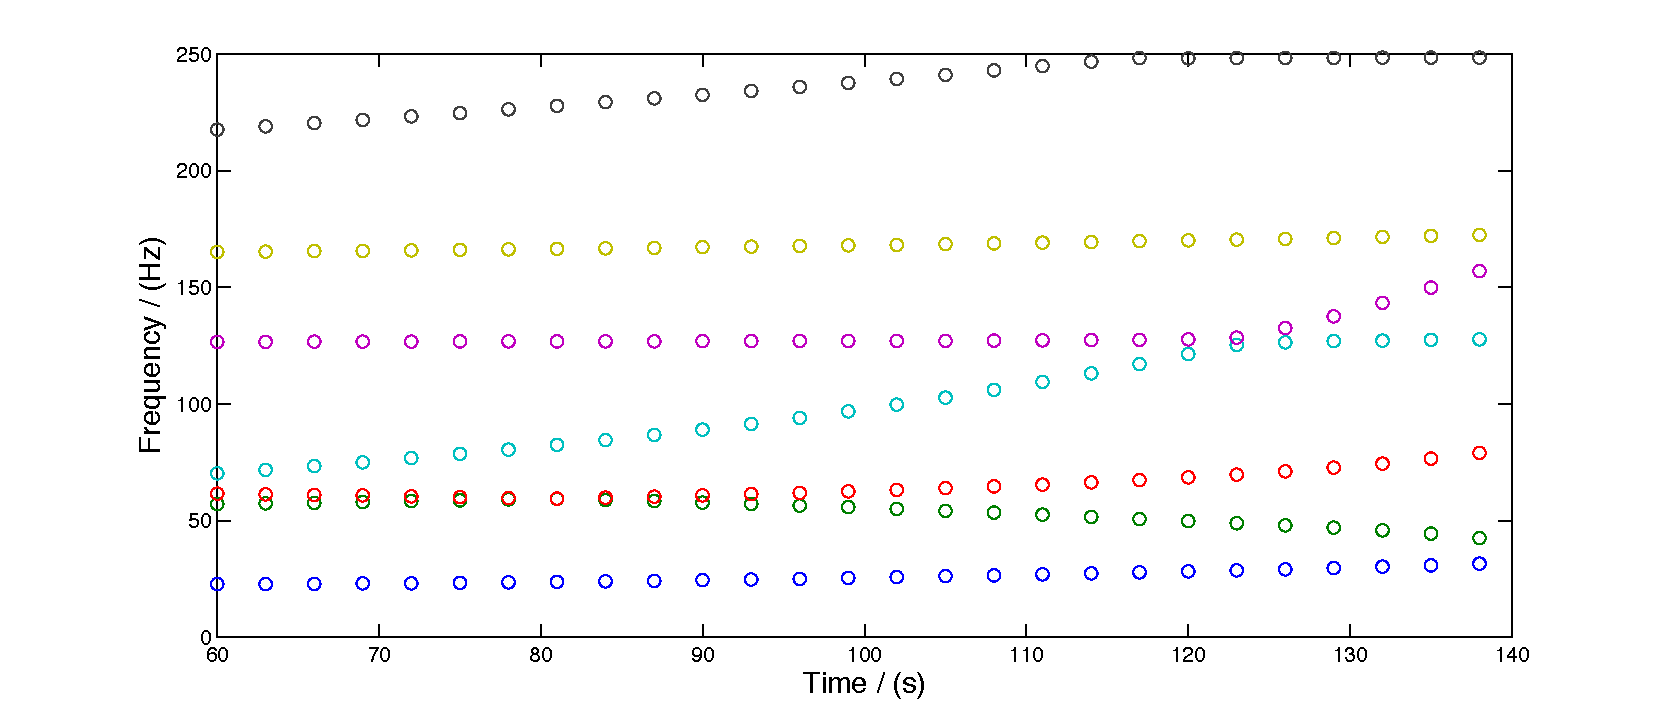
\includegraphics[trim={1.5cm 0cm 1.5cm 0cm}, clip=true, width=.92\linewidth]{Lumped-Frequency-Curve.pdf}
  \caption{耦合系统集中参数模型的固有频率变化曲线}\label{Lumped-Frequency-Curve}
\end{figure}

\begin{figure}[!htb]
  \centering
  %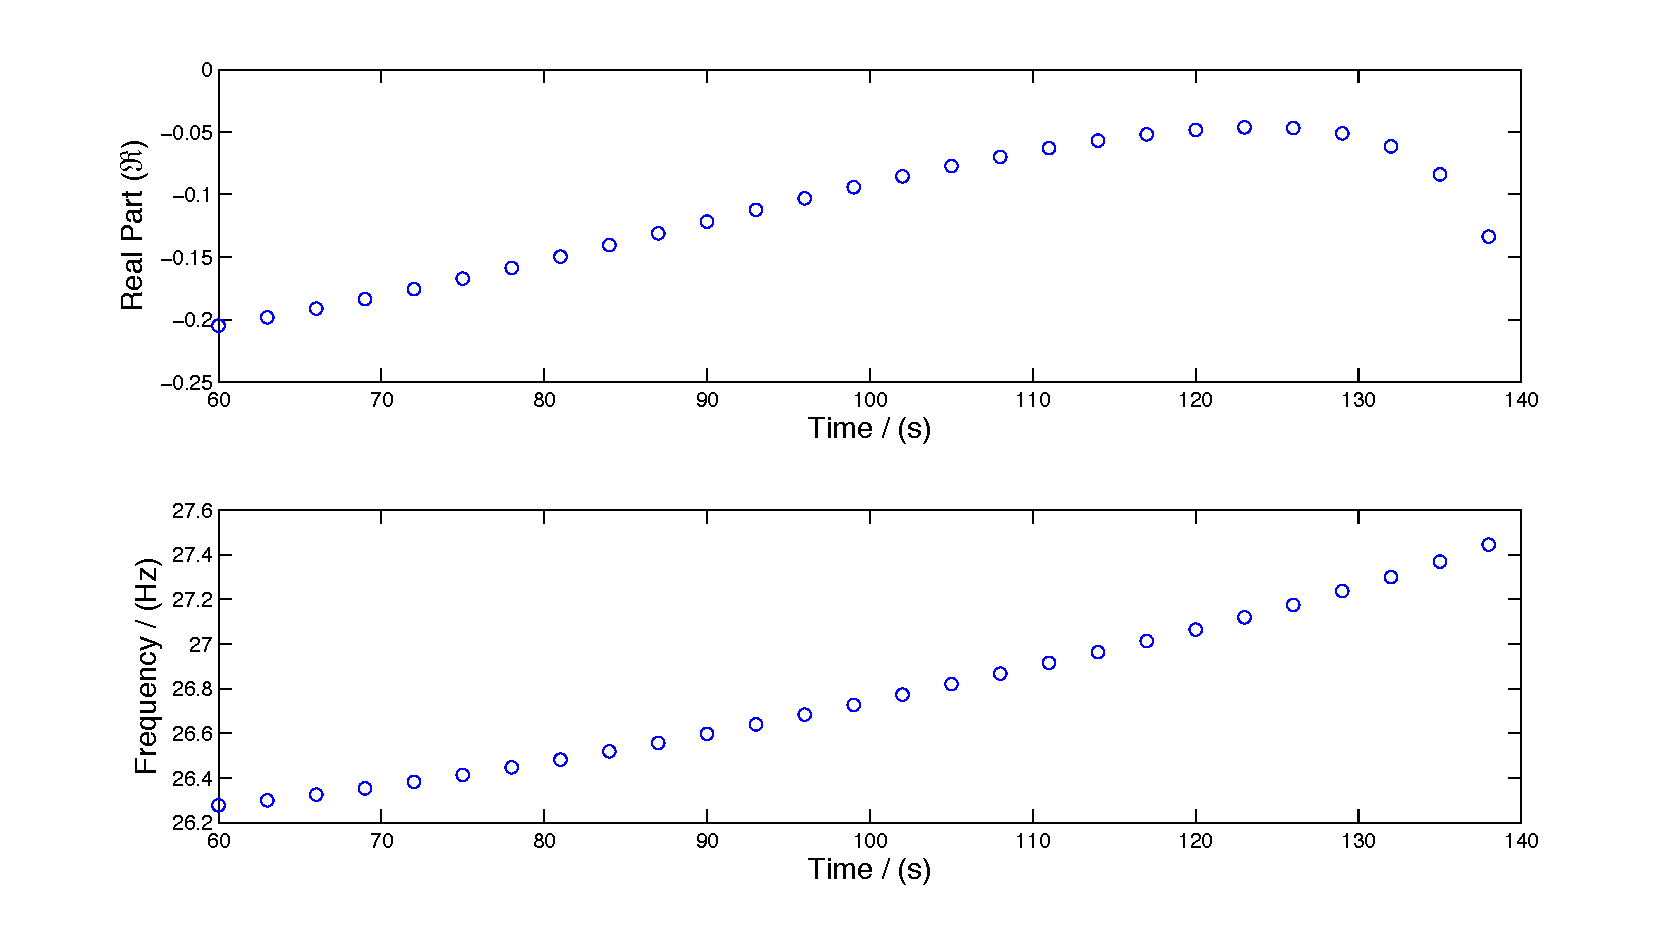
\includegraphics[trim={1.5cm 0.4cm 1.5cm 1cm}, clip=true, width=.92\linewidth]{Lumped-Max-Eigen-Curve.pdf}
  \caption{耦合系统集中参数模型的特征值变化曲线}\label{Lumped-Max-Eigen-Curve}
\end{figure}

\bibliographystyle{FDUbib}
\bibliography{ref}









